\documentclass[twoside]{book}

% Packages required by doxygen
\usepackage{fixltx2e}
\usepackage{calc}
\usepackage{doxygen}
\usepackage[export]{adjustbox} % also loads graphicx
\usepackage{graphicx}
\usepackage[utf8]{inputenc}
\usepackage{makeidx}
\usepackage{multicol}
\usepackage{multirow}
\PassOptionsToPackage{warn}{textcomp}
\usepackage{textcomp}
\usepackage[nointegrals]{wasysym}
\usepackage[table]{xcolor}

% Font selection
\usepackage[T1]{fontenc}
\usepackage[scaled=.90]{helvet}
\usepackage{courier}
\usepackage{amssymb}
\usepackage{sectsty}
\renewcommand{\familydefault}{\sfdefault}
\allsectionsfont{%
  \fontseries{bc}\selectfont%
  \color{darkgray}%
}
\renewcommand{\DoxyLabelFont}{%
  \fontseries{bc}\selectfont%
  \color{darkgray}%
}
\newcommand{\+}{\discretionary{\mbox{\scriptsize$\hookleftarrow$}}{}{}}

% Page & text layout
\usepackage{geometry}
\geometry{%
  a4paper,%
  top=2.5cm,%
  bottom=2.5cm,%
  left=2.5cm,%
  right=2.5cm%
}
\tolerance=750
\hfuzz=15pt
\hbadness=750
\setlength{\emergencystretch}{15pt}
\setlength{\parindent}{0cm}
\setlength{\parskip}{3ex plus 2ex minus 2ex}
\makeatletter
\renewcommand{\paragraph}{%
  \@startsection{paragraph}{4}{0ex}{-1.0ex}{1.0ex}{%
    \normalfont\normalsize\bfseries\SS@parafont%
  }%
}
\renewcommand{\subparagraph}{%
  \@startsection{subparagraph}{5}{0ex}{-1.0ex}{1.0ex}{%
    \normalfont\normalsize\bfseries\SS@subparafont%
  }%
}
\makeatother

% Headers & footers
\usepackage{fancyhdr}
\pagestyle{fancyplain}
\fancyhead[LE]{\fancyplain{}{\bfseries\thepage}}
\fancyhead[CE]{\fancyplain{}{}}
\fancyhead[RE]{\fancyplain{}{\bfseries\leftmark}}
\fancyhead[LO]{\fancyplain{}{\bfseries\rightmark}}
\fancyhead[CO]{\fancyplain{}{}}
\fancyhead[RO]{\fancyplain{}{\bfseries\thepage}}
\fancyfoot[LE]{\fancyplain{}{}}
\fancyfoot[CE]{\fancyplain{}{}}
\fancyfoot[RE]{\fancyplain{}{\bfseries\scriptsize Generated by Doxygen }}
\fancyfoot[LO]{\fancyplain{}{\bfseries\scriptsize Generated by Doxygen }}
\fancyfoot[CO]{\fancyplain{}{}}
\fancyfoot[RO]{\fancyplain{}{}}
\renewcommand{\footrulewidth}{0.4pt}
\renewcommand{\chaptermark}[1]{%
  \markboth{#1}{}%
}
\renewcommand{\sectionmark}[1]{%
  \markright{\thesection\ #1}%
}

% Indices & bibliography
\usepackage{natbib}
\usepackage[titles]{tocloft}
\setcounter{tocdepth}{3}
\setcounter{secnumdepth}{5}
\makeindex

% Hyperlinks (required, but should be loaded last)
\usepackage{ifpdf}
\ifpdf
  \usepackage[pdftex,pagebackref=true]{hyperref}
\else
  \usepackage[ps2pdf,pagebackref=true]{hyperref}
\fi
\hypersetup{%
  colorlinks=true,%
  linkcolor=blue,%
  citecolor=blue,%
  unicode%
}

% Custom commands
\newcommand{\clearemptydoublepage}{%
  \newpage{\pagestyle{empty}\cleardoublepage}%
}

\usepackage{caption}
\captionsetup{labelsep=space,justification=centering,font={bf},singlelinecheck=off,skip=4pt,position=top}

%===== C O N T E N T S =====

\begin{document}

% Titlepage & ToC
\hypersetup{pageanchor=false,
             bookmarksnumbered=true,
             pdfencoding=unicode
            }
\pagenumbering{alph}
\begin{titlepage}
\vspace*{7cm}
\begin{center}%
{\Large Library\+Mathematics \\[1ex]\large 2018.\+06.\+25 }\\
\vspace*{1cm}
{\large Generated by Doxygen 1.8.13}\\
\end{center}
\end{titlepage}
\clearemptydoublepage
\pagenumbering{roman}
\tableofcontents
\clearemptydoublepage
\pagenumbering{arabic}
\hypersetup{pageanchor=true}

%--- Begin generated contents ---
\chapter{Library \+:\+: Mathematics}
\label{index}\hypertarget{index}{}Geometry, curve fitting, optimization.

\href{https://travis-ci.com/open-space-collective/library-mathematics}{\tt } \href{https://codecov.io/gh/open-space-collective/library-mathematics}{\tt } \href{https://open-space-collective.github.io/library-mathematics}{\tt } \href{https://badge.fury.io/gh/open-space-collective%2Flibrary-mathematics}{\tt } \href{https://badge.fury.io/py/LibraryMathematicsPy}{\tt }

\subsection*{Warning}

Library {\bfseries name} and {\bfseries license} are yet to be defined.

Please check the following projects\+:


\begin{DoxyItemize}
\item \href{https://github.com/orgs/open-space-collective/projects/1}{\tt Naming Project}
\item \href{https://github.com/orgs/open-space-collective/projects/2}{\tt Licensing Project}
\end{DoxyItemize}

{\itshape ⚠ This library is still under heavy development. Do not use!}

\subsection*{Structure}

The {\bfseries Mathematics} library exhibits the following structure\+:


\begin{DoxyCode}
├── Objects
│   ├── Vector
│   ├── Matrix
│   └── Interval
├── Geometry
│   ├── 2D
|   │   ├── Objects
│   │   │   ├── Point
│   │   │   ├── Point Set
│   │   │   ├── Line
│   │   │   ├── Line String
│   │   │   ├── Multi Line String
│   │   │   └── Polygon
│   │   ├── Intersection
│   │   └── Transformations
│   │       ├── Identity
│   │       ├── Translation
│   │       ├── Rotation
│   │       ├── Reflection
│   │       ├── Scaling
│   │       └── Shear
│   ├── 3D
|   │   ├── Objects
│   │   │   ├── Point
│   │   │   ├── Point Set
│   │   │   ├── Line
│   │   │   ├── Ray
│   │   │   ├── Segment
│   │   │   ├── Rectangle
│   │   │   ├── Plane
│   │   │   ├── Sphere
│   │   │   ├── Ellipsoid
│   │   │   ├── Cone
│   │   │   └── Pyramid
│   │   ├── Intersection
│   │   └── Transformations
│   │       ├── Identity
│   │       ├── Translation
│   │       ├── Rotations
│   │       │   ├── Quaternion
│   │       │   ├── Euler Angle
│   │       │   ├── Rotation Vector
│   │       │   └── Rotation Matrix
│   │       ├── Reflection
│   │       ├── Scaling
│   │       └── Shear
├── Dynamics
│   ├── State
│   ├── Solvers
│   │   ├── Runge–Kutta 4 (RK4)
│   │   ├── Dormand–Prince 5 (DP5)
│   │   └── Runge–Kutta–Fehlberg 78 (F78)
│   └── Systems
├── Curve Fitting
│   ├── Interpolation
│   │   ├── Linear
│   │   ├── Cubic Spline
│   │   └── Lagrange
│   └── Smoothing
├── Optimization
│   ├── Problem
│   └── Algorithms
│       ├── Gradient Descent
│       └── Evolutionary
│           ├── Genetic
│           ├── Differential Evolution
│           └── Swarm
└── Statistics
\end{DoxyCode}


\subsection*{Documentation}

The documentation can be found here\+:


\begin{DoxyItemize}
\item \href{https://open-space-collective.github.io/library-mathematics}{\tt C++}
\item \href{./bindings/python/docs}{\tt Python}
\end{DoxyItemize}

\subsection*{Tutorials}

Various tutorials are available here\+:


\begin{DoxyItemize}
\item \href{./tutorials/cpp}{\tt C++}
\item \href{./tutorials/python}{\tt Python}
\end{DoxyItemize}

\subsection*{Setup}

\subsubsection*{Development}

Using \href{https://www.docker.com}{\tt Docker} is recommended, as the development tools and dependencies setup is described in the provided \href{./tools/development/docker/Dockerfile}{\tt Dockerfile}.

Instructions to install Docker can be found \href{https://docs.docker.com/install/}{\tt here}.

Start the development environment\+:


\begin{DoxyCode}
./tools/development/start.sh
\end{DoxyCode}


This will also build the {\ttfamily openspacecollective/library-\/mathematics\+:latest} Docker image, if not already.

If installing Docker is not an option, please manually install the development tools (G\+CC, C\+Make) and the dependencies. The procedure should be similar to the one described in the \href{./tools/development/docker/Dockerfile}{\tt Dockerfile}.

\subsubsection*{Build}

From the development environment\+:


\begin{DoxyCode}
./build.sh
\end{DoxyCode}


Manually\+:


\begin{DoxyCode}
mkdir -p build
cd build
cmake ..
make
\end{DoxyCode}


\subsubsection*{Test}

From the development environment\+:


\begin{DoxyCode}
./test.sh
\end{DoxyCode}


Manually\+:


\begin{DoxyCode}
./bin/library-mathematics.test
\end{DoxyCode}


\subsection*{Dependencies}

The {\bfseries Mathematics} library internally uses the following dependencies\+:

\tabulinesep=1mm
\begin{longtabu} spread 0pt [c]{*{4}{|X[-1]}|}
\hline
\rowcolor{\tableheadbgcolor}\textbf{ Name }&\textbf{ Version }&\textbf{ License }&\textbf{ Link  }\\\cline{1-4}
\endfirsthead
\hline
\endfoot
\hline
\rowcolor{\tableheadbgcolor}\textbf{ Name }&\textbf{ Version }&\textbf{ License }&\textbf{ Link  }\\\cline{1-4}
\endhead
Boost &1.\+67.\+0 &Boost Software License &\href{https://www.boost.org}{\tt boost.\+org} \\\cline{1-4}
Eigen &3.\+3.\+4 &M\+P\+L2 &\href{http://eigen.tuxfamily.org/index.php}{\tt eigen.\+tuxfamily.\+org} \\\cline{1-4}
Geometric Tools Engine &3.\+14 &Boost Software License &\href{https://www.geometrictools.com}{\tt geometrictools.\+com} \\\cline{1-4}
Core &master &T\+BD &\href{https://github.com/open-space-collective/library-core}{\tt github.\+com/open-\/space-\/collective/library-\/core} \\\cline{1-4}
\end{longtabu}
\subsection*{Contribution}

Contributions are more than welcome!

Please read our \hyperlink{_c_o_n_t_r_i_b_u_t_i_n_g_8md}{contributing guide} to learn about our development process, how to propose fixes and improvements, and how to build and test the code.

\subsection*{Special Thanks}

{\itshape To be completed...}

\subsection*{License}

{\itshape To be defined...} 
\chapter{Contributing}
\label{md__c_o_n_t_r_i_b_u_t_i_n_g}
\Hypertarget{md__c_o_n_t_r_i_b_u_t_i_n_g}
{\itshape ⚠ This document is a work in progress.}\hypertarget{md__c_o_n_t_r_i_b_u_t_i_n_g_Introduction}{}\section{Introduction}\label{md__c_o_n_t_r_i_b_u_t_i_n_g_Introduction}
{\itshape To be completed...}\hypertarget{md__c_o_n_t_r_i_b_u_t_i_n_g_Guidelines}{}\section{Guidelines}\label{md__c_o_n_t_r_i_b_u_t_i_n_g_Guidelines}
\hypertarget{md__c_o_n_t_r_i_b_u_t_i_n_g_Codebase}{}\subsection{Codebase}\label{md__c_o_n_t_r_i_b_u_t_i_n_g_Codebase}
\hypertarget{md__c_o_n_t_r_i_b_u_t_i_n_g_C}{}\subsubsection{C++}\label{md__c_o_n_t_r_i_b_u_t_i_n_g_C}
Include order from specific to generic\+:


\begin{DoxyCode}
\textcolor{preprocessor}{#include <Library/Astrodynamics/Orbit.hpp>}

\textcolor{preprocessor}{#include <Library/Core/Types/Integer.hpp>}
\textcolor{preprocessor}{#include <Library/Core/Utilities.hpp>}

\textcolor{preprocessor}{#include <map>}
\textcolor{preprocessor}{#include <string>}
\end{DoxyCode}


References\+:


\begin{DoxyItemize}
\item \href{https://stackoverflow.com/questions/2762568/c-c-include-file-order-best-practices}{\tt https\+://stackoverflow.\+com/questions/2762568/c-\/c-\/include-\/file-\/order-\/best-\/practices}
\item \href{https://blog.kowalczyk.info/article/qg/order-of-include-headers-in-cc.html}{\tt https\+://blog.\+kowalczyk.\+info/article/qg/order-\/of-\/include-\/headers-\/in-\/cc.\+html}
\end{DoxyItemize}\hypertarget{md__c_o_n_t_r_i_b_u_t_i_n_g_Python}{}\subsubsection{Python}\label{md__c_o_n_t_r_i_b_u_t_i_n_g_Python}
{\itshape To be completed...}\hypertarget{md__c_o_n_t_r_i_b_u_t_i_n_g_Version}{}\subsection{Version Control}\label{md__c_o_n_t_r_i_b_u_t_i_n_g_Version}
\hypertarget{md__c_o_n_t_r_i_b_u_t_i_n_g_Rules}{}\subsubsection{Rules}\label{md__c_o_n_t_r_i_b_u_t_i_n_g_Rules}
{\itshape To be completed...}\hypertarget{md__c_o_n_t_r_i_b_u_t_i_n_g_Commit}{}\subsubsection{Commit Messages}\label{md__c_o_n_t_r_i_b_u_t_i_n_g_Commit}
\href{https://chris.beams.io/posts/git-commit/}{\tt How to Write a Git Commit Message}

Use active form ({\ttfamily Do something}).

Prefix commit messages using the following tags\+:


\begin{DoxyItemize}
\item \mbox{[}feature\mbox{]}
\item \mbox{[}fix\mbox{]}
\item \mbox{[}misc\mbox{]}
\end{DoxyItemize}

Examples\+:


\begin{DoxyCode}
[feature] Implement high fidelity orbit propagator
\end{DoxyCode}



\begin{DoxyCode}
[fix] Segmentation fault when fetching ephemeris data
\end{DoxyCode}
\hypertarget{md__c_o_n_t_r_i_b_u_t_i_n_g_CodeOfConduct}{}\section{Code of Conduct}\label{md__c_o_n_t_r_i_b_u_t_i_n_g_CodeOfConduct}
{\itshape To be completed...} 
\chapter{Tutorial}
\label{md_docs__tutorial}
\Hypertarget{md_docs__tutorial}
Below are examples illustrating a few common use-\/cases.\hypertarget{md_docs__tutorial_Setup}{}\section{Setup}\label{md_docs__tutorial_Setup}
{\itshape To be completed...}\hypertarget{md_docs__tutorial_Examples}{}\section{Examples}\label{md_docs__tutorial_Examples}
{\itshape To be completed...} 
\chapter{Namespace Index}
\section{Namespace List}
Here is a list of all namespaces with brief descriptions\+:\begin{DoxyCompactList}
\item\contentsline{section}{\hyperlink{namespacelibrary}{library} }{\pageref{namespacelibrary}}{}
\item\contentsline{section}{\hyperlink{namespacelibrary_1_1math}{library\+::math} }{\pageref{namespacelibrary_1_1math}}{}
\item\contentsline{section}{\hyperlink{namespacelibrary_1_1math_1_1obj}{library\+::math\+::obj} }{\pageref{namespacelibrary_1_1math_1_1obj}}{}
\item\contentsline{section}{\hyperlink{namespacelibrary_1_1math_1_1trf}{library\+::math\+::trf} }{\pageref{namespacelibrary_1_1math_1_1trf}}{}
\item\contentsline{section}{\hyperlink{namespacelibrary_1_1math_1_1trf_1_1rot}{library\+::math\+::trf\+::rot} }{\pageref{namespacelibrary_1_1math_1_1trf_1_1rot}}{}
\end{DoxyCompactList}

\chapter{Class Index}
\section{Class List}
Here are the classes, structs, unions and interfaces with brief descriptions\+:\begin{DoxyCompactList}
\item\contentsline{section}{\hyperlink{classlibrary_1_1math_1_1geom_1_1_angle}{library\+::math\+::geom\+::\+Angle} \\*\hyperlink{classlibrary_1_1math_1_1geom_1_1_angle}{Angle} }{\pageref{classlibrary_1_1math_1_1geom_1_1_angle}}{}
\item\contentsline{section}{\hyperlink{classlibrary_1_1math_1_1geom_1_1d3_1_1objects_1_1_composite}{library\+::math\+::geom\+::d3\+::objects\+::\+Composite} \\*\hyperlink{classlibrary_1_1math_1_1geom_1_1d3_1_1objects_1_1_composite}{Composite} object }{\pageref{classlibrary_1_1math_1_1geom_1_1d3_1_1objects_1_1_composite}}{}
\item\contentsline{section}{\hyperlink{classlibrary_1_1math_1_1geom_1_1d3_1_1objects_1_1_cuboid}{library\+::math\+::geom\+::d3\+::objects\+::\+Cuboid} \\*\hyperlink{classlibrary_1_1math_1_1geom_1_1d3_1_1objects_1_1_cuboid}{Cuboid} }{\pageref{classlibrary_1_1math_1_1geom_1_1d3_1_1objects_1_1_cuboid}}{}
\item\contentsline{section}{\hyperlink{classlibrary_1_1math_1_1geom_1_1d3_1_1objects_1_1_ellipsoid}{library\+::math\+::geom\+::d3\+::objects\+::\+Ellipsoid} \\*\hyperlink{classlibrary_1_1math_1_1geom_1_1d3_1_1objects_1_1_ellipsoid}{Ellipsoid} }{\pageref{classlibrary_1_1math_1_1geom_1_1d3_1_1objects_1_1_ellipsoid}}{}
\item\contentsline{section}{\hyperlink{structlibrary_1_1math_1_1geom_1_1d2_1_1objects_1_1_point_set_1_1_hasher}{library\+::math\+::geom\+::d2\+::objects\+::\+Point\+Set\+::\+Hasher} \\*\hyperlink{classlibrary_1_1math_1_1geom_1_1d2_1_1objects_1_1_point}{Point} hasher }{\pageref{structlibrary_1_1math_1_1geom_1_1d2_1_1objects_1_1_point_set_1_1_hasher}}{}
\item\contentsline{section}{\hyperlink{structlibrary_1_1math_1_1geom_1_1d3_1_1objects_1_1_point_set_1_1_hasher}{library\+::math\+::geom\+::d3\+::objects\+::\+Point\+Set\+::\+Hasher} \\*\hyperlink{classlibrary_1_1math_1_1geom_1_1d3_1_1objects_1_1_point}{Point} hasher }{\pageref{structlibrary_1_1math_1_1geom_1_1d3_1_1objects_1_1_point_set_1_1_hasher}}{}
\item\contentsline{section}{\hyperlink{classlibrary_1_1math_1_1geom_1_1d3_1_1_intersection}{library\+::math\+::geom\+::d3\+::\+Intersection} \\*3D intersection }{\pageref{classlibrary_1_1math_1_1geom_1_1d3_1_1_intersection}}{}
\item\contentsline{section}{\hyperlink{classlibrary_1_1math_1_1obj_1_1_interval}{library\+::math\+::obj\+::\+Interval$<$ T $>$} \\*Set of numbers with the property that any number that lies between two numbers in the set is also included in the set }{\pageref{classlibrary_1_1math_1_1obj_1_1_interval}}{}
\item\contentsline{section}{\hyperlink{classlibrary_1_1math_1_1obj_1_1_interval_base}{library\+::math\+::obj\+::\+Interval\+Base} \\*\hyperlink{classlibrary_1_1math_1_1obj_1_1_interval}{Interval} base (used to avoid having a templated enum) }{\pageref{classlibrary_1_1math_1_1obj_1_1_interval_base}}{}
\item\contentsline{section}{\hyperlink{classlibrary_1_1math_1_1geom_1_1d3_1_1objects_1_1_line}{library\+::math\+::geom\+::d3\+::objects\+::\+Line} \\*\hyperlink{classlibrary_1_1math_1_1geom_1_1d3_1_1objects_1_1_line}{Line} }{\pageref{classlibrary_1_1math_1_1geom_1_1d3_1_1objects_1_1_line}}{}
\item\contentsline{section}{\hyperlink{classlibrary_1_1math_1_1geom_1_1d3_1_1objects_1_1_line_string}{library\+::math\+::geom\+::d3\+::objects\+::\+Line\+String} \\*\hyperlink{classlibrary_1_1math_1_1geom_1_1d3_1_1objects_1_1_line}{Line} string }{\pageref{classlibrary_1_1math_1_1geom_1_1d3_1_1objects_1_1_line_string}}{}
\item\contentsline{section}{\hyperlink{classlibrary_1_1math_1_1geom_1_1d2_1_1objects_1_1_line_string}{library\+::math\+::geom\+::d2\+::objects\+::\+Line\+String} \\*Line string }{\pageref{classlibrary_1_1math_1_1geom_1_1d2_1_1objects_1_1_line_string}}{}
\item\contentsline{section}{\hyperlink{classlibrary_1_1math_1_1geom_1_1d2_1_1objects_1_1_multi_line_string}{library\+::math\+::geom\+::d2\+::objects\+::\+Multi\+Line\+String} \\*Multi Line string }{\pageref{classlibrary_1_1math_1_1geom_1_1d2_1_1objects_1_1_multi_line_string}}{}
\item\contentsline{section}{\hyperlink{classlibrary_1_1math_1_1geom_1_1d2_1_1_object}{library\+::math\+::geom\+::d2\+::\+Object} \\*2D object }{\pageref{classlibrary_1_1math_1_1geom_1_1d2_1_1_object}}{}
\item\contentsline{section}{\hyperlink{classlibrary_1_1math_1_1geom_1_1d3_1_1_object}{library\+::math\+::geom\+::d3\+::\+Object} \\*3D object }{\pageref{classlibrary_1_1math_1_1geom_1_1d3_1_1_object}}{}
\item\contentsline{section}{\hyperlink{classlibrary_1_1math_1_1geom_1_1d3_1_1objects_1_1_plane}{library\+::math\+::geom\+::d3\+::objects\+::\+Plane} \\*\hyperlink{classlibrary_1_1math_1_1geom_1_1d3_1_1objects_1_1_plane}{Plane} }{\pageref{classlibrary_1_1math_1_1geom_1_1d3_1_1objects_1_1_plane}}{}
\item\contentsline{section}{\hyperlink{classlibrary_1_1math_1_1geom_1_1d2_1_1objects_1_1_point}{library\+::math\+::geom\+::d2\+::objects\+::\+Point} \\*\hyperlink{classlibrary_1_1math_1_1geom_1_1d2_1_1objects_1_1_point}{Point} }{\pageref{classlibrary_1_1math_1_1geom_1_1d2_1_1objects_1_1_point}}{}
\item\contentsline{section}{\hyperlink{classlibrary_1_1math_1_1geom_1_1d3_1_1objects_1_1_point}{library\+::math\+::geom\+::d3\+::objects\+::\+Point} \\*\hyperlink{classlibrary_1_1math_1_1geom_1_1d3_1_1objects_1_1_point}{Point} }{\pageref{classlibrary_1_1math_1_1geom_1_1d3_1_1objects_1_1_point}}{}
\item\contentsline{section}{\hyperlink{classlibrary_1_1math_1_1geom_1_1d3_1_1objects_1_1_point_set}{library\+::math\+::geom\+::d3\+::objects\+::\+Point\+Set} \\*\hyperlink{classlibrary_1_1math_1_1geom_1_1d3_1_1objects_1_1_point}{Point} set }{\pageref{classlibrary_1_1math_1_1geom_1_1d3_1_1objects_1_1_point_set}}{}
\item\contentsline{section}{\hyperlink{classlibrary_1_1math_1_1geom_1_1d2_1_1objects_1_1_point_set}{library\+::math\+::geom\+::d2\+::objects\+::\+Point\+Set} \\*\hyperlink{classlibrary_1_1math_1_1geom_1_1d2_1_1objects_1_1_point}{Point} set }{\pageref{classlibrary_1_1math_1_1geom_1_1d2_1_1objects_1_1_point_set}}{}
\item\contentsline{section}{\hyperlink{classlibrary_1_1math_1_1geom_1_1d2_1_1objects_1_1_polygon}{library\+::math\+::geom\+::d2\+::objects\+::\+Polygon} \\*\hyperlink{classlibrary_1_1math_1_1geom_1_1d2_1_1objects_1_1_polygon}{Polygon} }{\pageref{classlibrary_1_1math_1_1geom_1_1d2_1_1objects_1_1_polygon}}{}
\item\contentsline{section}{\hyperlink{classlibrary_1_1math_1_1geom_1_1d3_1_1objects_1_1_polygon}{library\+::math\+::geom\+::d3\+::objects\+::\+Polygon} \\*\hyperlink{classlibrary_1_1math_1_1geom_1_1d3_1_1objects_1_1_polygon}{Polygon} }{\pageref{classlibrary_1_1math_1_1geom_1_1d3_1_1objects_1_1_polygon}}{}
\item\contentsline{section}{\hyperlink{classlibrary_1_1math_1_1geom_1_1d3_1_1objects_1_1_pyramid}{library\+::math\+::geom\+::d3\+::objects\+::\+Pyramid} \\*\hyperlink{classlibrary_1_1math_1_1geom_1_1d3_1_1objects_1_1_pyramid}{Pyramid} }{\pageref{classlibrary_1_1math_1_1geom_1_1d3_1_1objects_1_1_pyramid}}{}
\item\contentsline{section}{\hyperlink{classlibrary_1_1math_1_1geom_1_1d3_1_1trf_1_1rot_1_1_quaternion}{library\+::math\+::geom\+::d3\+::trf\+::rot\+::\+Quaternion} \\*\hyperlink{classlibrary_1_1math_1_1geom_1_1d3_1_1trf_1_1rot_1_1_quaternion}{Quaternion} }{\pageref{classlibrary_1_1math_1_1geom_1_1d3_1_1trf_1_1rot_1_1_quaternion}}{}
\item\contentsline{section}{\hyperlink{classlibrary_1_1math_1_1geom_1_1d3_1_1objects_1_1_ray}{library\+::math\+::geom\+::d3\+::objects\+::\+Ray} \\*\hyperlink{classlibrary_1_1math_1_1geom_1_1d3_1_1objects_1_1_ray}{Ray} }{\pageref{classlibrary_1_1math_1_1geom_1_1d3_1_1objects_1_1_ray}}{}
\item\contentsline{section}{\hyperlink{classlibrary_1_1math_1_1geom_1_1d3_1_1trf_1_1rot_1_1_rotation_matrix}{library\+::math\+::geom\+::d3\+::trf\+::rot\+::\+Rotation\+Matrix} \\*Rotation matrix }{\pageref{classlibrary_1_1math_1_1geom_1_1d3_1_1trf_1_1rot_1_1_rotation_matrix}}{}
\item\contentsline{section}{\hyperlink{classlibrary_1_1math_1_1geom_1_1d3_1_1trf_1_1rot_1_1_rotation_vector}{library\+::math\+::geom\+::d3\+::trf\+::rot\+::\+Rotation\+Vector} \\*Rotation vector }{\pageref{classlibrary_1_1math_1_1geom_1_1d3_1_1trf_1_1rot_1_1_rotation_vector}}{}
\item\contentsline{section}{\hyperlink{classlibrary_1_1math_1_1geom_1_1d2_1_1objects_1_1_segment}{library\+::math\+::geom\+::d2\+::objects\+::\+Segment} \\*\hyperlink{classlibrary_1_1math_1_1geom_1_1d2_1_1objects_1_1_segment}{Segment} }{\pageref{classlibrary_1_1math_1_1geom_1_1d2_1_1objects_1_1_segment}}{}
\item\contentsline{section}{\hyperlink{classlibrary_1_1math_1_1geom_1_1d3_1_1objects_1_1_segment}{library\+::math\+::geom\+::d3\+::objects\+::\+Segment} \\*\hyperlink{classlibrary_1_1math_1_1geom_1_1d3_1_1objects_1_1_segment}{Segment} }{\pageref{classlibrary_1_1math_1_1geom_1_1d3_1_1objects_1_1_segment}}{}
\item\contentsline{section}{\hyperlink{classlibrary_1_1math_1_1geom_1_1d3_1_1objects_1_1_sphere}{library\+::math\+::geom\+::d3\+::objects\+::\+Sphere} \\*\hyperlink{classlibrary_1_1math_1_1geom_1_1d3_1_1objects_1_1_sphere}{Sphere} }{\pageref{classlibrary_1_1math_1_1geom_1_1d3_1_1objects_1_1_sphere}}{}
\item\contentsline{section}{\hyperlink{classlibrary_1_1math_1_1geom_1_1d3_1_1_transformation}{library\+::math\+::geom\+::d3\+::\+Transformation} }{\pageref{classlibrary_1_1math_1_1geom_1_1d3_1_1_transformation}}{}
\item\contentsline{section}{\hyperlink{classlibrary_1_1math_1_1geom_1_1d2_1_1_transformation}{library\+::math\+::geom\+::d2\+::\+Transformation} }{\pageref{classlibrary_1_1math_1_1geom_1_1d2_1_1_transformation}}{}
\end{DoxyCompactList}

\chapter{File Index}
\section{File List}
Here is a list of all files with brief descriptions\+:\begin{DoxyCompactList}
\item\contentsline{section}{include/\+Library/\+Mathematics/\hyperlink{_objects_8hpp}{Objects.\+hpp} }{\pageref{_objects_8hpp}}{}
\item\contentsline{section}{include/\+Library/\+Mathematics/\+Geometry/\hyperlink{_angle_8hpp}{Angle.\+hpp} }{\pageref{_angle_8hpp}}{}
\item\contentsline{section}{include/\+Library/\+Mathematics/\+Geometry/\hyperlink{_transformation_8hpp}{Transformation.\+hpp} }{\pageref{_transformation_8hpp}}{}
\item\contentsline{section}{include/\+Library/\+Mathematics/\+Geometry/2\+D/\hyperlink{2_d_2_object_8hpp}{Object.\+hpp} }{\pageref{2_d_2_object_8hpp}}{}
\item\contentsline{section}{include/\+Library/\+Mathematics/\+Geometry/2\+D/\+Objects/\hyperlink{2_d_2_objects_2_point_8hpp}{Point.\+hpp} }{\pageref{2_d_2_objects_2_point_8hpp}}{}
\item\contentsline{section}{include/\+Library/\+Mathematics/\+Geometry/2\+D/\+Objects/\hyperlink{2_d_2_objects_2_polygon_8hpp}{Polygon.\+hpp} }{\pageref{2_d_2_objects_2_polygon_8hpp}}{}
\item\contentsline{section}{include/\+Library/\+Mathematics/\+Geometry/3\+D/\hyperlink{_intersection_8hpp}{Intersection.\+hpp} }{\pageref{_intersection_8hpp}}{}
\item\contentsline{section}{include/\+Library/\+Mathematics/\+Geometry/3\+D/\hyperlink{3_d_2_object_8hpp}{Object.\+hpp} }{\pageref{3_d_2_object_8hpp}}{}
\item\contentsline{section}{include/\+Library/\+Mathematics/\+Geometry/3\+D/\+Objects/\hyperlink{_ellipsoid_8hpp}{Ellipsoid.\+hpp} }{\pageref{_ellipsoid_8hpp}}{}
\item\contentsline{section}{include/\+Library/\+Mathematics/\+Geometry/3\+D/\+Objects/\hyperlink{_plane_8hpp}{Plane.\+hpp} }{\pageref{_plane_8hpp}}{}
\item\contentsline{section}{include/\+Library/\+Mathematics/\+Geometry/3\+D/\+Objects/\hyperlink{3_d_2_objects_2_point_8hpp}{Point.\+hpp} }{\pageref{3_d_2_objects_2_point_8hpp}}{}
\item\contentsline{section}{include/\+Library/\+Mathematics/\+Geometry/3\+D/\+Objects/\hyperlink{3_d_2_objects_2_polygon_8hpp}{Polygon.\+hpp} }{\pageref{3_d_2_objects_2_polygon_8hpp}}{}
\item\contentsline{section}{include/\+Library/\+Mathematics/\+Geometry/3\+D/\+Objects/\hyperlink{_pyramid_8hpp}{Pyramid.\+hpp} }{\pageref{_pyramid_8hpp}}{}
\item\contentsline{section}{include/\+Library/\+Mathematics/\+Geometry/3\+D/\+Objects/\hyperlink{_segment_8hpp}{Segment.\+hpp} }{\pageref{_segment_8hpp}}{}
\item\contentsline{section}{include/\+Library/\+Mathematics/\+Geometry/3\+D/\+Objects/\hyperlink{_sphere_8hpp}{Sphere.\+hpp} }{\pageref{_sphere_8hpp}}{}
\item\contentsline{section}{include/\+Library/\+Mathematics/\+Geometry/\+Transformations/\+Rotations/\hyperlink{_euler_angle_8hpp}{Euler\+Angle.\+hpp} }{\pageref{_euler_angle_8hpp}}{}
\item\contentsline{section}{include/\+Library/\+Mathematics/\+Geometry/\+Transformations/\+Rotations/\hyperlink{_quaternion_8hpp}{Quaternion.\+hpp} }{\pageref{_quaternion_8hpp}}{}
\item\contentsline{section}{include/\+Library/\+Mathematics/\+Geometry/\+Transformations/\+Rotations/\hyperlink{_rotation_matrix_8hpp}{Rotation\+Matrix.\+hpp} }{\pageref{_rotation_matrix_8hpp}}{}
\item\contentsline{section}{include/\+Library/\+Mathematics/\+Geometry/\+Transformations/\+Rotations/\hyperlink{_rotation_vector_8hpp}{Rotation\+Vector.\+hpp} }{\pageref{_rotation_vector_8hpp}}{}
\item\contentsline{section}{include/\+Library/\+Mathematics/\+Objects/\hyperlink{_eigen_8hpp}{Eigen.\+hpp} }{\pageref{_eigen_8hpp}}{}
\item\contentsline{section}{include/\+Library/\+Mathematics/\+Objects/\hyperlink{_interval_8hpp}{Interval.\+hpp} }{\pageref{_interval_8hpp}}{}
\item\contentsline{section}{include/\+Library/\+Mathematics/\+Objects/\hyperlink{_matrix_8hpp}{Matrix.\+hpp} }{\pageref{_matrix_8hpp}}{}
\item\contentsline{section}{include/\+Library/\+Mathematics/\+Objects/\hyperlink{_vector_8hpp}{Vector.\+hpp} }{\pageref{_vector_8hpp}}{}
\item\contentsline{section}{src/\+Library/\+Mathematics/\+Geometry/\hyperlink{_angle_8cpp}{Angle.\+cpp} }{\pageref{_angle_8cpp}}{}
\item\contentsline{section}{src/\+Library/\+Mathematics/\+Geometry/2\+D/\hyperlink{2_d_2_object_8cpp}{Object.\+cpp} }{\pageref{2_d_2_object_8cpp}}{}
\item\contentsline{section}{src/\+Library/\+Mathematics/\+Geometry/2\+D/\+Objects/\hyperlink{2_d_2_objects_2_point_8cpp}{Point.\+cpp} }{\pageref{2_d_2_objects_2_point_8cpp}}{}
\item\contentsline{section}{src/\+Library/\+Mathematics/\+Geometry/2\+D/\+Objects/\hyperlink{_polygon_8cpp}{Polygon.\+cpp} }{\pageref{_polygon_8cpp}}{}
\item\contentsline{section}{src/\+Library/\+Mathematics/\+Geometry/3\+D/\hyperlink{_intersection_8cpp}{Intersection.\+cpp} }{\pageref{_intersection_8cpp}}{}
\item\contentsline{section}{src/\+Library/\+Mathematics/\+Geometry/3\+D/\hyperlink{3_d_2_object_8cpp}{Object.\+cpp} }{\pageref{3_d_2_object_8cpp}}{}
\item\contentsline{section}{src/\+Library/\+Mathematics/\+Geometry/3\+D/\+Objects/\hyperlink{_ellipsoid_8cpp}{Ellipsoid.\+cpp} }{\pageref{_ellipsoid_8cpp}}{}
\item\contentsline{section}{src/\+Library/\+Mathematics/\+Geometry/3\+D/\+Objects/\hyperlink{3_d_2_objects_2_point_8cpp}{Point.\+cpp} }{\pageref{3_d_2_objects_2_point_8cpp}}{}
\item\contentsline{section}{src/\+Library/\+Mathematics/\+Geometry/3\+D/\+Objects/\hyperlink{_segment_8cpp}{Segment.\+cpp} }{\pageref{_segment_8cpp}}{}
\item\contentsline{section}{src/\+Library/\+Mathematics/\+Geometry/3\+D/\+Objects/\hyperlink{_sphere_8cpp}{Sphere.\+cpp} }{\pageref{_sphere_8cpp}}{}
\item\contentsline{section}{src/\+Library/\+Mathematics/\+Geometry/\+Transformations/\+Rotations/\hyperlink{_quaternion_8cpp}{Quaternion.\+cpp} }{\pageref{_quaternion_8cpp}}{}
\item\contentsline{section}{src/\+Library/\+Mathematics/\+Geometry/\+Transformations/\+Rotations/\hyperlink{_rotation_matrix_8cpp}{Rotation\+Matrix.\+cpp} }{\pageref{_rotation_matrix_8cpp}}{}
\item\contentsline{section}{src/\+Library/\+Mathematics/\+Geometry/\+Transformations/\+Rotations/\hyperlink{_rotation_vector_8cpp}{Rotation\+Vector.\+cpp} }{\pageref{_rotation_vector_8cpp}}{}
\item\contentsline{section}{src/\+Library/\+Mathematics/\+Objects/\hyperlink{_interval_8tpp}{Interval.\+tpp} }{\pageref{_interval_8tpp}}{}
\item\contentsline{section}{src/\+Library/\+Mathematics/\+Objects/\hyperlink{_matrix_8cpp}{Matrix.\+cpp} }{\pageref{_matrix_8cpp}}{}
\item\contentsline{section}{src/\+Library/\+Mathematics/\+Objects/\hyperlink{_vector_8cpp}{Vector.\+cpp} }{\pageref{_vector_8cpp}}{}
\end{DoxyCompactList}

\chapter{Namespace Documentation}
\hypertarget{namespacelibrary}{}\section{library Namespace Reference}
\label{namespacelibrary}\index{library@{library}}
\subsection*{Namespaces}
\begin{DoxyCompactItemize}
\item 
 \hyperlink{namespacelibrary_1_1math}{math}
\end{DoxyCompactItemize}

\hypertarget{namespacelibrary_1_1math}{}\section{library\+:\+:math Namespace Reference}
\label{namespacelibrary_1_1math}\index{library\+::math@{library\+::math}}
\subsection*{Namespaces}
\begin{DoxyCompactItemize}
\item 
 \hyperlink{namespacelibrary_1_1math_1_1obj}{obj}
\item 
 \hyperlink{namespacelibrary_1_1math_1_1trf}{trf}
\end{DoxyCompactItemize}

\hypertarget{namespacelibrary_1_1math_1_1obj}{}\section{library\+:\+:math\+:\+:obj Namespace Reference}
\label{namespacelibrary_1_1math_1_1obj}\index{library\+::math\+::obj@{library\+::math\+::obj}}
\subsection*{Classes}
\begin{DoxyCompactItemize}
\item 
class \hyperlink{classlibrary_1_1math_1_1obj_1_1_interval}{Interval}
\begin{DoxyCompactList}\small\item\em Set of numbers with the property that any number that lies between two numbers in the set is also included in the set. \end{DoxyCompactList}\item 
class \hyperlink{classlibrary_1_1math_1_1obj_1_1_interval_base}{Interval\+Base}
\begin{DoxyCompactList}\small\item\em \hyperlink{classlibrary_1_1math_1_1obj_1_1_interval}{Interval} base (used to avoid having a templated enum) \end{DoxyCompactList}\end{DoxyCompactItemize}
\subsection*{Typedefs}
\begin{DoxyCompactItemize}
\item 
using \hyperlink{namespacelibrary_1_1math_1_1obj_a27d8117bb406c37fd0aee60b61f0bcb9}{Vector2i} = Eigen\+::\+Vector2i
\item 
using \hyperlink{namespacelibrary_1_1math_1_1obj_a9d2ecef9029409b29e79b366e0b9941f}{Vector3i} = Eigen\+::\+Vector3i
\item 
using \hyperlink{namespacelibrary_1_1math_1_1obj_a5181dbb9520bc27fe956555569ef1271}{Vector4i} = Eigen\+::\+Vector4i
\item 
using \hyperlink{namespacelibrary_1_1math_1_1obj_a2cd4b891130c163c72ea6a546132cb2d}{Vector\+Xi} = Eigen\+::\+Vector\+Xi
\item 
using \hyperlink{namespacelibrary_1_1math_1_1obj_a2fa27512c4f4b07db35d602cfdd2c293}{Vector2d} = Eigen\+::\+Vector2d
\item 
using \hyperlink{namespacelibrary_1_1math_1_1obj_a977e84e9bf317a4e7dd9d6d671d6da2f}{Vector3d} = Eigen\+::\+Vector3d
\item 
using \hyperlink{namespacelibrary_1_1math_1_1obj_a5679bbebea773cc0d4ed6ec28eb79c03}{Vector4d} = Eigen\+::\+Vector4d
\item 
using \hyperlink{namespacelibrary_1_1math_1_1obj_a54fa1a789b235483252f0525f0abf579}{Vector\+Xd} = Eigen\+::\+Vector\+Xd
\item 
using \hyperlink{namespacelibrary_1_1math_1_1obj_a0ece80fce95e1fdaeea8b3e232b45765}{Row\+Vector\+Xd} = Eigen\+::\+Row\+Vector\+Xd
\item 
using \hyperlink{namespacelibrary_1_1math_1_1obj_abd4bcf17b090b90261299f718df7fd50}{Matrix2i} = Eigen\+::\+Matrix2i
\item 
using \hyperlink{namespacelibrary_1_1math_1_1obj_a7e74feec88408f948fe6d4a18d274619}{Matrix3i} = Eigen\+::\+Matrix3i
\item 
using \hyperlink{namespacelibrary_1_1math_1_1obj_af485a47cffc7369c6b462b1a58b4db60}{Matrix4i} = Eigen\+::\+Matrix4i
\item 
using \hyperlink{namespacelibrary_1_1math_1_1obj_a3b9388d308b3ea0f1f8fe9b9dedaed0c}{Matrix\+Xi} = Eigen\+::\+Matrix\+Xi
\item 
using \hyperlink{namespacelibrary_1_1math_1_1obj_a967d79db25d723ff05600d29055be7b9}{Matrix2d} = Eigen\+::\+Matrix2d
\item 
using \hyperlink{namespacelibrary_1_1math_1_1obj_a49dc66c2ba45a70c9fcef7aa03ba0b42}{Matrix3d} = Eigen\+::\+Matrix3d
\item 
using \hyperlink{namespacelibrary_1_1math_1_1obj_adde130f80968bf89120e5ff29929bfed}{Matrix4d} = Eigen\+::\+Matrix4d
\item 
using \hyperlink{namespacelibrary_1_1math_1_1obj_a4da50132532e4544429d239909ccbd79}{Matrix\+Xd} = Eigen\+::\+Matrix\+Xd
\end{DoxyCompactItemize}


\subsection{Typedef Documentation}
\mbox{\Hypertarget{namespacelibrary_1_1math_1_1obj_a967d79db25d723ff05600d29055be7b9}\label{namespacelibrary_1_1math_1_1obj_a967d79db25d723ff05600d29055be7b9}} 
\index{library\+::math\+::obj@{library\+::math\+::obj}!Matrix2d@{Matrix2d}}
\index{Matrix2d@{Matrix2d}!library\+::math\+::obj@{library\+::math\+::obj}}
\subsubsection{\texorpdfstring{Matrix2d}{Matrix2d}}
{\footnotesize\ttfamily using \hyperlink{namespacelibrary_1_1math_1_1obj_a967d79db25d723ff05600d29055be7b9}{library\+::math\+::obj\+::\+Matrix2d} = typedef Eigen\+::\+Matrix2d}

\mbox{\Hypertarget{namespacelibrary_1_1math_1_1obj_abd4bcf17b090b90261299f718df7fd50}\label{namespacelibrary_1_1math_1_1obj_abd4bcf17b090b90261299f718df7fd50}} 
\index{library\+::math\+::obj@{library\+::math\+::obj}!Matrix2i@{Matrix2i}}
\index{Matrix2i@{Matrix2i}!library\+::math\+::obj@{library\+::math\+::obj}}
\subsubsection{\texorpdfstring{Matrix2i}{Matrix2i}}
{\footnotesize\ttfamily using \hyperlink{namespacelibrary_1_1math_1_1obj_abd4bcf17b090b90261299f718df7fd50}{library\+::math\+::obj\+::\+Matrix2i} = typedef Eigen\+::\+Matrix2i}

\mbox{\Hypertarget{namespacelibrary_1_1math_1_1obj_a49dc66c2ba45a70c9fcef7aa03ba0b42}\label{namespacelibrary_1_1math_1_1obj_a49dc66c2ba45a70c9fcef7aa03ba0b42}} 
\index{library\+::math\+::obj@{library\+::math\+::obj}!Matrix3d@{Matrix3d}}
\index{Matrix3d@{Matrix3d}!library\+::math\+::obj@{library\+::math\+::obj}}
\subsubsection{\texorpdfstring{Matrix3d}{Matrix3d}}
{\footnotesize\ttfamily using \hyperlink{namespacelibrary_1_1math_1_1obj_a49dc66c2ba45a70c9fcef7aa03ba0b42}{library\+::math\+::obj\+::\+Matrix3d} = typedef Eigen\+::\+Matrix3d}

\mbox{\Hypertarget{namespacelibrary_1_1math_1_1obj_a7e74feec88408f948fe6d4a18d274619}\label{namespacelibrary_1_1math_1_1obj_a7e74feec88408f948fe6d4a18d274619}} 
\index{library\+::math\+::obj@{library\+::math\+::obj}!Matrix3i@{Matrix3i}}
\index{Matrix3i@{Matrix3i}!library\+::math\+::obj@{library\+::math\+::obj}}
\subsubsection{\texorpdfstring{Matrix3i}{Matrix3i}}
{\footnotesize\ttfamily using \hyperlink{namespacelibrary_1_1math_1_1obj_a7e74feec88408f948fe6d4a18d274619}{library\+::math\+::obj\+::\+Matrix3i} = typedef Eigen\+::\+Matrix3i}

\mbox{\Hypertarget{namespacelibrary_1_1math_1_1obj_adde130f80968bf89120e5ff29929bfed}\label{namespacelibrary_1_1math_1_1obj_adde130f80968bf89120e5ff29929bfed}} 
\index{library\+::math\+::obj@{library\+::math\+::obj}!Matrix4d@{Matrix4d}}
\index{Matrix4d@{Matrix4d}!library\+::math\+::obj@{library\+::math\+::obj}}
\subsubsection{\texorpdfstring{Matrix4d}{Matrix4d}}
{\footnotesize\ttfamily using \hyperlink{namespacelibrary_1_1math_1_1obj_adde130f80968bf89120e5ff29929bfed}{library\+::math\+::obj\+::\+Matrix4d} = typedef Eigen\+::\+Matrix4d}

\mbox{\Hypertarget{namespacelibrary_1_1math_1_1obj_af485a47cffc7369c6b462b1a58b4db60}\label{namespacelibrary_1_1math_1_1obj_af485a47cffc7369c6b462b1a58b4db60}} 
\index{library\+::math\+::obj@{library\+::math\+::obj}!Matrix4i@{Matrix4i}}
\index{Matrix4i@{Matrix4i}!library\+::math\+::obj@{library\+::math\+::obj}}
\subsubsection{\texorpdfstring{Matrix4i}{Matrix4i}}
{\footnotesize\ttfamily using \hyperlink{namespacelibrary_1_1math_1_1obj_af485a47cffc7369c6b462b1a58b4db60}{library\+::math\+::obj\+::\+Matrix4i} = typedef Eigen\+::\+Matrix4i}

\mbox{\Hypertarget{namespacelibrary_1_1math_1_1obj_a4da50132532e4544429d239909ccbd79}\label{namespacelibrary_1_1math_1_1obj_a4da50132532e4544429d239909ccbd79}} 
\index{library\+::math\+::obj@{library\+::math\+::obj}!Matrix\+Xd@{Matrix\+Xd}}
\index{Matrix\+Xd@{Matrix\+Xd}!library\+::math\+::obj@{library\+::math\+::obj}}
\subsubsection{\texorpdfstring{Matrix\+Xd}{MatrixXd}}
{\footnotesize\ttfamily using \hyperlink{namespacelibrary_1_1math_1_1obj_a4da50132532e4544429d239909ccbd79}{library\+::math\+::obj\+::\+Matrix\+Xd} = typedef Eigen\+::\+Matrix\+Xd}

\mbox{\Hypertarget{namespacelibrary_1_1math_1_1obj_a3b9388d308b3ea0f1f8fe9b9dedaed0c}\label{namespacelibrary_1_1math_1_1obj_a3b9388d308b3ea0f1f8fe9b9dedaed0c}} 
\index{library\+::math\+::obj@{library\+::math\+::obj}!Matrix\+Xi@{Matrix\+Xi}}
\index{Matrix\+Xi@{Matrix\+Xi}!library\+::math\+::obj@{library\+::math\+::obj}}
\subsubsection{\texorpdfstring{Matrix\+Xi}{MatrixXi}}
{\footnotesize\ttfamily using \hyperlink{namespacelibrary_1_1math_1_1obj_a3b9388d308b3ea0f1f8fe9b9dedaed0c}{library\+::math\+::obj\+::\+Matrix\+Xi} = typedef Eigen\+::\+Matrix\+Xi}

\mbox{\Hypertarget{namespacelibrary_1_1math_1_1obj_a0ece80fce95e1fdaeea8b3e232b45765}\label{namespacelibrary_1_1math_1_1obj_a0ece80fce95e1fdaeea8b3e232b45765}} 
\index{library\+::math\+::obj@{library\+::math\+::obj}!Row\+Vector\+Xd@{Row\+Vector\+Xd}}
\index{Row\+Vector\+Xd@{Row\+Vector\+Xd}!library\+::math\+::obj@{library\+::math\+::obj}}
\subsubsection{\texorpdfstring{Row\+Vector\+Xd}{RowVectorXd}}
{\footnotesize\ttfamily using \hyperlink{namespacelibrary_1_1math_1_1obj_a0ece80fce95e1fdaeea8b3e232b45765}{library\+::math\+::obj\+::\+Row\+Vector\+Xd} = typedef Eigen\+::\+Row\+Vector\+Xd}

\mbox{\Hypertarget{namespacelibrary_1_1math_1_1obj_a2fa27512c4f4b07db35d602cfdd2c293}\label{namespacelibrary_1_1math_1_1obj_a2fa27512c4f4b07db35d602cfdd2c293}} 
\index{library\+::math\+::obj@{library\+::math\+::obj}!Vector2d@{Vector2d}}
\index{Vector2d@{Vector2d}!library\+::math\+::obj@{library\+::math\+::obj}}
\subsubsection{\texorpdfstring{Vector2d}{Vector2d}}
{\footnotesize\ttfamily using \hyperlink{namespacelibrary_1_1math_1_1obj_a2fa27512c4f4b07db35d602cfdd2c293}{library\+::math\+::obj\+::\+Vector2d} = typedef Eigen\+::\+Vector2d}

\mbox{\Hypertarget{namespacelibrary_1_1math_1_1obj_a27d8117bb406c37fd0aee60b61f0bcb9}\label{namespacelibrary_1_1math_1_1obj_a27d8117bb406c37fd0aee60b61f0bcb9}} 
\index{library\+::math\+::obj@{library\+::math\+::obj}!Vector2i@{Vector2i}}
\index{Vector2i@{Vector2i}!library\+::math\+::obj@{library\+::math\+::obj}}
\subsubsection{\texorpdfstring{Vector2i}{Vector2i}}
{\footnotesize\ttfamily using \hyperlink{namespacelibrary_1_1math_1_1obj_a27d8117bb406c37fd0aee60b61f0bcb9}{library\+::math\+::obj\+::\+Vector2i} = typedef Eigen\+::\+Vector2i}

\mbox{\Hypertarget{namespacelibrary_1_1math_1_1obj_a977e84e9bf317a4e7dd9d6d671d6da2f}\label{namespacelibrary_1_1math_1_1obj_a977e84e9bf317a4e7dd9d6d671d6da2f}} 
\index{library\+::math\+::obj@{library\+::math\+::obj}!Vector3d@{Vector3d}}
\index{Vector3d@{Vector3d}!library\+::math\+::obj@{library\+::math\+::obj}}
\subsubsection{\texorpdfstring{Vector3d}{Vector3d}}
{\footnotesize\ttfamily using \hyperlink{namespacelibrary_1_1math_1_1obj_a977e84e9bf317a4e7dd9d6d671d6da2f}{library\+::math\+::obj\+::\+Vector3d} = typedef Eigen\+::\+Vector3d}

\mbox{\Hypertarget{namespacelibrary_1_1math_1_1obj_a9d2ecef9029409b29e79b366e0b9941f}\label{namespacelibrary_1_1math_1_1obj_a9d2ecef9029409b29e79b366e0b9941f}} 
\index{library\+::math\+::obj@{library\+::math\+::obj}!Vector3i@{Vector3i}}
\index{Vector3i@{Vector3i}!library\+::math\+::obj@{library\+::math\+::obj}}
\subsubsection{\texorpdfstring{Vector3i}{Vector3i}}
{\footnotesize\ttfamily using \hyperlink{namespacelibrary_1_1math_1_1obj_a9d2ecef9029409b29e79b366e0b9941f}{library\+::math\+::obj\+::\+Vector3i} = typedef Eigen\+::\+Vector3i}

\mbox{\Hypertarget{namespacelibrary_1_1math_1_1obj_a5679bbebea773cc0d4ed6ec28eb79c03}\label{namespacelibrary_1_1math_1_1obj_a5679bbebea773cc0d4ed6ec28eb79c03}} 
\index{library\+::math\+::obj@{library\+::math\+::obj}!Vector4d@{Vector4d}}
\index{Vector4d@{Vector4d}!library\+::math\+::obj@{library\+::math\+::obj}}
\subsubsection{\texorpdfstring{Vector4d}{Vector4d}}
{\footnotesize\ttfamily using \hyperlink{namespacelibrary_1_1math_1_1obj_a5679bbebea773cc0d4ed6ec28eb79c03}{library\+::math\+::obj\+::\+Vector4d} = typedef Eigen\+::\+Vector4d}

\mbox{\Hypertarget{namespacelibrary_1_1math_1_1obj_a5181dbb9520bc27fe956555569ef1271}\label{namespacelibrary_1_1math_1_1obj_a5181dbb9520bc27fe956555569ef1271}} 
\index{library\+::math\+::obj@{library\+::math\+::obj}!Vector4i@{Vector4i}}
\index{Vector4i@{Vector4i}!library\+::math\+::obj@{library\+::math\+::obj}}
\subsubsection{\texorpdfstring{Vector4i}{Vector4i}}
{\footnotesize\ttfamily using \hyperlink{namespacelibrary_1_1math_1_1obj_a5181dbb9520bc27fe956555569ef1271}{library\+::math\+::obj\+::\+Vector4i} = typedef Eigen\+::\+Vector4i}

\mbox{\Hypertarget{namespacelibrary_1_1math_1_1obj_a54fa1a789b235483252f0525f0abf579}\label{namespacelibrary_1_1math_1_1obj_a54fa1a789b235483252f0525f0abf579}} 
\index{library\+::math\+::obj@{library\+::math\+::obj}!Vector\+Xd@{Vector\+Xd}}
\index{Vector\+Xd@{Vector\+Xd}!library\+::math\+::obj@{library\+::math\+::obj}}
\subsubsection{\texorpdfstring{Vector\+Xd}{VectorXd}}
{\footnotesize\ttfamily using \hyperlink{namespacelibrary_1_1math_1_1obj_a54fa1a789b235483252f0525f0abf579}{library\+::math\+::obj\+::\+Vector\+Xd} = typedef Eigen\+::\+Vector\+Xd}

\mbox{\Hypertarget{namespacelibrary_1_1math_1_1obj_a2cd4b891130c163c72ea6a546132cb2d}\label{namespacelibrary_1_1math_1_1obj_a2cd4b891130c163c72ea6a546132cb2d}} 
\index{library\+::math\+::obj@{library\+::math\+::obj}!Vector\+Xi@{Vector\+Xi}}
\index{Vector\+Xi@{Vector\+Xi}!library\+::math\+::obj@{library\+::math\+::obj}}
\subsubsection{\texorpdfstring{Vector\+Xi}{VectorXi}}
{\footnotesize\ttfamily using \hyperlink{namespacelibrary_1_1math_1_1obj_a2cd4b891130c163c72ea6a546132cb2d}{library\+::math\+::obj\+::\+Vector\+Xi} = typedef Eigen\+::\+Vector\+Xi}


\hypertarget{namespacelibrary_1_1math_1_1trf}{}\section{library\+:\+:math\+:\+:trf Namespace Reference}
\label{namespacelibrary_1_1math_1_1trf}\index{library\+::math\+::trf@{library\+::math\+::trf}}
\subsection*{Namespaces}
\begin{DoxyCompactItemize}
\item 
 \hyperlink{namespacelibrary_1_1math_1_1trf_1_1rot}{rot}
\end{DoxyCompactItemize}

\hypertarget{namespacelibrary_1_1math_1_1trf_1_1rot}{}\section{library\+:\+:math\+:\+:trf\+:\+:rot Namespace Reference}
\label{namespacelibrary_1_1math_1_1trf_1_1rot}\index{library\+::math\+::trf\+::rot@{library\+::math\+::trf\+::rot}}

\chapter{Class Documentation}
\hypertarget{classlibrary_1_1math_1_1obj_1_1_interval}{}\section{library\+:\+:math\+:\+:obj\+:\+:Interval$<$ T $>$ Class Template Reference}
\label{classlibrary_1_1math_1_1obj_1_1_interval}\index{library\+::math\+::obj\+::\+Interval$<$ T $>$@{library\+::math\+::obj\+::\+Interval$<$ T $>$}}


Set of numbers with the property that any number that lies between two numbers in the set is also included in the set.  




{\ttfamily \#include $<$Interval.\+hpp$>$}

Inheritance diagram for library\+:\+:math\+:\+:obj\+:\+:Interval$<$ T $>$\+:\begin{figure}[H]
\begin{center}
\leavevmode
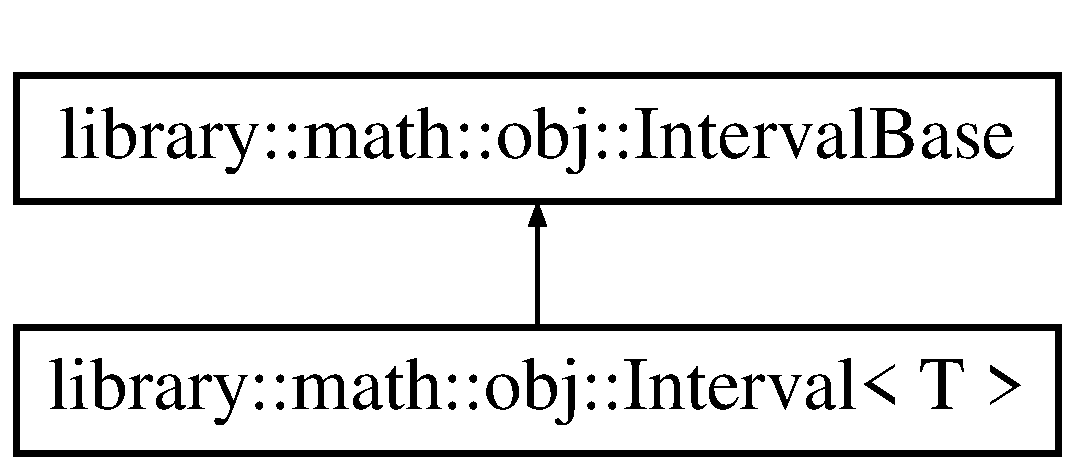
\includegraphics[height=2.000000cm]{classlibrary_1_1math_1_1obj_1_1_interval}
\end{center}
\end{figure}
\subsection*{Public Member Functions}
\begin{DoxyCompactItemize}
\item 
\hyperlink{classlibrary_1_1math_1_1obj_1_1_interval_ad3c3506ca4e90506ab1ea25a18fc5cd7}{Interval} (const T \&a\+Lower\+Bound, const T \&an\+Upper\+Bound, const \hyperlink{classlibrary_1_1math_1_1obj_1_1_interval_base_aabce6fa07a6e2e8fd3fcab5fd0d317d6}{Interval\+::\+Type} \&an\+Interval\+Type)
\begin{DoxyCompactList}\small\item\em Constructor. \end{DoxyCompactList}\item 
bool \hyperlink{classlibrary_1_1math_1_1obj_1_1_interval_a99b12768e33b75bf87ab656b92c03e98}{operator==} (const \hyperlink{classlibrary_1_1math_1_1obj_1_1_interval}{Interval} \&an\+Interval) const
\begin{DoxyCompactList}\small\item\em Equal to operator. \end{DoxyCompactList}\item 
bool \hyperlink{classlibrary_1_1math_1_1obj_1_1_interval_a5ca4c08ba0aff1ea42ea3804d51e02cf}{operator!=} (const \hyperlink{classlibrary_1_1math_1_1obj_1_1_interval}{Interval} \&an\+Interval) const
\begin{DoxyCompactList}\small\item\em Not equal to operator. \end{DoxyCompactList}\item 
bool \hyperlink{classlibrary_1_1math_1_1obj_1_1_interval_a2de37bb9d7b97ae7892188c26c99b6fb}{is\+Defined} () const
\begin{DoxyCompactList}\small\item\em Check if interval is defined. \end{DoxyCompactList}\item 
bool \hyperlink{classlibrary_1_1math_1_1obj_1_1_interval_a0e9997639f0c415f4f7fe8dcb58e13a8}{is\+Degenerate} () const
\begin{DoxyCompactList}\small\item\em Check if interval is degenerate, i.\+e. its lower and upper bounds are the equal. \end{DoxyCompactList}\item 
bool \hyperlink{classlibrary_1_1math_1_1obj_1_1_interval_aba618feb6e4b6d052999c2b8c8c0b06a}{intersects} (const \hyperlink{classlibrary_1_1math_1_1obj_1_1_interval}{Interval} \&an\+Interval) const
\begin{DoxyCompactList}\small\item\em Check if interval is intersecting with another interval. \end{DoxyCompactList}\item 
bool \hyperlink{classlibrary_1_1math_1_1obj_1_1_interval_af100f4b53dc3211efde2733c19e458c3}{contains} (const T \&a\+Value) const
\begin{DoxyCompactList}\small\item\em Check if interval contains value. \end{DoxyCompactList}\item 
bool \hyperlink{classlibrary_1_1math_1_1obj_1_1_interval_a3bace75e3cfb5f5c737e642c08572d25}{contains} (const \hyperlink{classlibrary_1_1math_1_1obj_1_1_interval}{Interval} \&an\+Interval) const
\begin{DoxyCompactList}\small\item\em Check if interval contains another interval. \end{DoxyCompactList}\item 
const T \& \hyperlink{classlibrary_1_1math_1_1obj_1_1_interval_ada0dc68134cfacd5a0e959b492cea534}{access\+Lower\+Bound} () const
\begin{DoxyCompactList}\small\item\em Get reference to lower bound. \end{DoxyCompactList}\item 
const T \& \hyperlink{classlibrary_1_1math_1_1obj_1_1_interval_a99692ee706ae6de7cd274ceae3644138}{access\+Upper\+Bound} () const
\begin{DoxyCompactList}\small\item\em Get reference to upper bound. \end{DoxyCompactList}\item 
\hyperlink{classlibrary_1_1math_1_1obj_1_1_interval_base_aabce6fa07a6e2e8fd3fcab5fd0d317d6}{Interval\+::\+Type} \hyperlink{classlibrary_1_1math_1_1obj_1_1_interval_a881ab7e17883b4f1553d7e8ba9cc7656}{get\+Type} () const
\begin{DoxyCompactList}\small\item\em Get interval type. \end{DoxyCompactList}\item 
T \hyperlink{classlibrary_1_1math_1_1obj_1_1_interval_a4e01721016dd02dddc93fb012ff7d5b3}{get\+Lower\+Bound} () const
\begin{DoxyCompactList}\small\item\em Get lower bound. \end{DoxyCompactList}\item 
T \hyperlink{classlibrary_1_1math_1_1obj_1_1_interval_a97d09e9c5e7f67b6ddf162af01a8066e}{get\+Upper\+Bound} () const
\begin{DoxyCompactList}\small\item\em Get upper bound. \end{DoxyCompactList}\item 
\hyperlink{classlibrary_1_1math_1_1obj_1_1_interval}{Interval}$<$ T $>$ \hyperlink{classlibrary_1_1math_1_1obj_1_1_interval_a2f23ca14d71c454417270218132423de}{get\+Intersection\+With} (const \hyperlink{classlibrary_1_1math_1_1obj_1_1_interval}{Interval} \&an\+Interval) const
\begin{DoxyCompactList}\small\item\em Get intersecting interval with another interval. \end{DoxyCompactList}\item 
\hyperlink{classlibrary_1_1math_1_1obj_1_1_interval}{Interval}$<$ T $>$ \hyperlink{classlibrary_1_1math_1_1obj_1_1_interval_a4183db388b6a63429a031d3687b20ecf}{get\+Union\+With} (const \hyperlink{classlibrary_1_1math_1_1obj_1_1_interval}{Interval} \&an\+Interval) const
\begin{DoxyCompactList}\small\item\em Get union interval with another interval. \end{DoxyCompactList}\item 
{\footnotesize template$<$class U $>$ }\\ctnr\+::\+Array$<$ T $>$ \hyperlink{classlibrary_1_1math_1_1obj_1_1_interval_ad453aeaec68c18421a7c93ac7c14fa48}{generate\+Array\+With\+Step} (const U \&a\+Step) const
\begin{DoxyCompactList}\small\item\em Generate array from a given step. \end{DoxyCompactList}\item 
ctnr\+::\+Array$<$ T $>$ \hyperlink{classlibrary_1_1math_1_1obj_1_1_interval_a250e05a1f463f107952b437e5ff4f4d2}{generate\+Array\+With\+Size} (const types\+::\+Size \&an\+Array\+Size) const
\begin{DoxyCompactList}\small\item\em Generate array with a given size. \end{DoxyCompactList}\item 
types\+::\+String \hyperlink{classlibrary_1_1math_1_1obj_1_1_interval_ad75c400daf533c35bc91da8c50b00a9e}{to\+String} () const
\begin{DoxyCompactList}\small\item\em Get serialized interval. \end{DoxyCompactList}\item 
void \hyperlink{classlibrary_1_1math_1_1obj_1_1_interval_a4dfb117d5a9c23bd32a3631fcf3686ec}{set\+Type} (const \hyperlink{classlibrary_1_1math_1_1obj_1_1_interval_base_aabce6fa07a6e2e8fd3fcab5fd0d317d6}{Interval\+::\+Type} \&a\+Type)
\begin{DoxyCompactList}\small\item\em \hyperlink{classlibrary_1_1math_1_1obj_1_1_interval}{Interval} type setter. \end{DoxyCompactList}\item 
void \hyperlink{classlibrary_1_1math_1_1obj_1_1_interval_a5ceb8fb56f920193c8b18346992b5d02}{set\+Lower\+Bound} (const T \&a\+Lower\+Bound)
\begin{DoxyCompactList}\small\item\em \hyperlink{classlibrary_1_1math_1_1obj_1_1_interval}{Interval} lower bound setter. \end{DoxyCompactList}\item 
void \hyperlink{classlibrary_1_1math_1_1obj_1_1_interval_a9c6b857d9fad97969635f669428c2b48}{set\+Upper\+Bound} (const T \&an\+Upper\+Bound)
\begin{DoxyCompactList}\small\item\em \hyperlink{classlibrary_1_1math_1_1obj_1_1_interval}{Interval} upper bound setter. \end{DoxyCompactList}\end{DoxyCompactItemize}
\subsection*{Static Public Member Functions}
\begin{DoxyCompactItemize}
\item 
static \hyperlink{classlibrary_1_1math_1_1obj_1_1_interval}{Interval}$<$ T $>$ \hyperlink{classlibrary_1_1math_1_1obj_1_1_interval_a415849a8c5306d6811612a842a5d0a40}{Undefined} ()
\begin{DoxyCompactList}\small\item\em Constructs an undefined interval. \end{DoxyCompactList}\item 
static \hyperlink{classlibrary_1_1math_1_1obj_1_1_interval}{Interval}$<$ T $>$ \hyperlink{classlibrary_1_1math_1_1obj_1_1_interval_aae8bb2b89af450729338d48563def4d7}{Closed} (const T \&a\+Lower\+Bound, const T \&an\+Upper\+Bound)
\begin{DoxyCompactList}\small\item\em Constructs a closed interval. \end{DoxyCompactList}\item 
static \hyperlink{classlibrary_1_1math_1_1obj_1_1_interval}{Interval}$<$ T $>$ \hyperlink{classlibrary_1_1math_1_1obj_1_1_interval_add0e1114a0c153da7a928fd059a08919}{Open} (const T \&a\+Lower\+Bound, const T \&an\+Upper\+Bound)
\begin{DoxyCompactList}\small\item\em Constructs an open interval. \end{DoxyCompactList}\item 
static \hyperlink{classlibrary_1_1math_1_1obj_1_1_interval}{Interval}$<$ T $>$ \hyperlink{classlibrary_1_1math_1_1obj_1_1_interval_a7e706c1e5133c731645e7633a9d763bd}{Half\+Open\+Left} (const T \&a\+Lower\+Bound, const T \&an\+Upper\+Bound)
\begin{DoxyCompactList}\small\item\em Constructs an half-\/open left interval. \end{DoxyCompactList}\item 
static \hyperlink{classlibrary_1_1math_1_1obj_1_1_interval}{Interval}$<$ T $>$ \hyperlink{classlibrary_1_1math_1_1obj_1_1_interval_a1a15d0518cc69fa3e442fc39c0622477}{Half\+Open\+Right} (const T \&a\+Lower\+Bound, const T \&an\+Upper\+Bound)
\begin{DoxyCompactList}\small\item\em Constructs an half-\/open right interval. \end{DoxyCompactList}\item 
static \hyperlink{classlibrary_1_1math_1_1obj_1_1_interval}{Interval}$<$ T $>$ \hyperlink{classlibrary_1_1math_1_1obj_1_1_interval_a9ed15c38ee04880a1aba75defa086a79}{Parse} (const types\+::\+String \&a\+String)
\begin{DoxyCompactList}\small\item\em Constructs an interval from a given string. \end{DoxyCompactList}\item 
static types\+::\+String \hyperlink{classlibrary_1_1math_1_1obj_1_1_interval_a64a1850152db9b95c9824c71378d9f40}{String\+From\+Type} (const \hyperlink{classlibrary_1_1math_1_1obj_1_1_interval_base_aabce6fa07a6e2e8fd3fcab5fd0d317d6}{Interval\+::\+Type} \&an\+Interval\+Type)
\begin{DoxyCompactList}\small\item\em Converts interval type to string. \end{DoxyCompactList}\end{DoxyCompactItemize}
\subsection*{Friends}
\begin{DoxyCompactItemize}
\item 
{\footnotesize template$<$class U $>$ }\\std\+::ostream \& \hyperlink{classlibrary_1_1math_1_1obj_1_1_interval_a3aa32afa8cb5d85eeb45540b0bf5657b}{operator$<$$<$} (std\+::ostream \&an\+Output\+Stream, const \hyperlink{classlibrary_1_1math_1_1obj_1_1_interval}{Interval}$<$ U $>$ \&an\+Interval)
\begin{DoxyCompactList}\small\item\em Output stream operator. \end{DoxyCompactList}\end{DoxyCompactItemize}
\subsection*{Additional Inherited Members}


\subsection{Detailed Description}
\subsubsection*{template$<$class T$>$\newline
class library\+::math\+::obj\+::\+Interval$<$ T $>$}

Set of numbers with the property that any number that lies between two numbers in the set is also included in the set. 

https\+://en.wikipedia.\+org/wiki/\+Interval\+\_\+(mathematics) 

\subsection{Constructor \& Destructor Documentation}
\mbox{\Hypertarget{classlibrary_1_1math_1_1obj_1_1_interval_ad3c3506ca4e90506ab1ea25a18fc5cd7}\label{classlibrary_1_1math_1_1obj_1_1_interval_ad3c3506ca4e90506ab1ea25a18fc5cd7}} 
\index{library\+::math\+::obj\+::\+Interval@{library\+::math\+::obj\+::\+Interval}!Interval@{Interval}}
\index{Interval@{Interval}!library\+::math\+::obj\+::\+Interval@{library\+::math\+::obj\+::\+Interval}}
\subsubsection{\texorpdfstring{Interval()}{Interval()}}
{\footnotesize\ttfamily template$<$class T$>$ \\
\hyperlink{classlibrary_1_1math_1_1obj_1_1_interval}{library\+::math\+::obj\+::\+Interval}$<$ T $>$\+::\hyperlink{classlibrary_1_1math_1_1obj_1_1_interval}{Interval} (\begin{DoxyParamCaption}\item[{const T \&}]{a\+Lower\+Bound,  }\item[{const T \&}]{an\+Upper\+Bound,  }\item[{const \hyperlink{classlibrary_1_1math_1_1obj_1_1_interval}{Interval}$<$ T $>$\+::\hyperlink{classlibrary_1_1math_1_1obj_1_1_interval_base_aabce6fa07a6e2e8fd3fcab5fd0d317d6}{Type} \&}]{an\+Interval\+Type }\end{DoxyParamCaption})}



Constructor. 


\begin{DoxyCode}
Interval<Real> interval(0.0, 1.0, \hyperlink{classlibrary_1_1math_1_1obj_1_1_interval_base_aabce6fa07a6e2e8fd3fcab5fd0d317d6a03f4a47830f97377a35321051685071e}{Interval::Type::Closed}) ;
\end{DoxyCode}



\begin{DoxyParams}[1]{Parameters}
\mbox{\tt in}  & {\em a\+Lower\+Bound} & A lower bound \\
\hline
\mbox{\tt in}  & {\em an\+Upper\+Bound} & An upper bound \\
\hline
\mbox{\tt in}  & {\em an\+Interval\+Type} & An interval type \\
\hline
\end{DoxyParams}


\subsection{Member Function Documentation}
\mbox{\Hypertarget{classlibrary_1_1math_1_1obj_1_1_interval_ada0dc68134cfacd5a0e959b492cea534}\label{classlibrary_1_1math_1_1obj_1_1_interval_ada0dc68134cfacd5a0e959b492cea534}} 
\index{library\+::math\+::obj\+::\+Interval@{library\+::math\+::obj\+::\+Interval}!access\+Lower\+Bound@{access\+Lower\+Bound}}
\index{access\+Lower\+Bound@{access\+Lower\+Bound}!library\+::math\+::obj\+::\+Interval@{library\+::math\+::obj\+::\+Interval}}
\subsubsection{\texorpdfstring{access\+Lower\+Bound()}{accessLowerBound()}}
{\footnotesize\ttfamily template$<$class T$>$ \\
const T\& \hyperlink{classlibrary_1_1math_1_1obj_1_1_interval}{library\+::math\+::obj\+::\+Interval}$<$ T $>$\+::access\+Lower\+Bound (\begin{DoxyParamCaption}{ }\end{DoxyParamCaption}) const}



Get reference to lower bound. 


\begin{DoxyCode}
Interval<Real> interval = \hyperlink{classlibrary_1_1math_1_1obj_1_1_interval_aae8bb2b89af450729338d48563def4d7}{Interval<Real>::Closed}(0.0, 1.0) ;
interval.accessLowerBound() ; \textcolor{comment}{// &0.0}
\end{DoxyCode}


\begin{DoxyReturn}{Returns}
Reference to lower bound 
\end{DoxyReturn}
\mbox{\Hypertarget{classlibrary_1_1math_1_1obj_1_1_interval_a99692ee706ae6de7cd274ceae3644138}\label{classlibrary_1_1math_1_1obj_1_1_interval_a99692ee706ae6de7cd274ceae3644138}} 
\index{library\+::math\+::obj\+::\+Interval@{library\+::math\+::obj\+::\+Interval}!access\+Upper\+Bound@{access\+Upper\+Bound}}
\index{access\+Upper\+Bound@{access\+Upper\+Bound}!library\+::math\+::obj\+::\+Interval@{library\+::math\+::obj\+::\+Interval}}
\subsubsection{\texorpdfstring{access\+Upper\+Bound()}{accessUpperBound()}}
{\footnotesize\ttfamily template$<$class T$>$ \\
const T\& \hyperlink{classlibrary_1_1math_1_1obj_1_1_interval}{library\+::math\+::obj\+::\+Interval}$<$ T $>$\+::access\+Upper\+Bound (\begin{DoxyParamCaption}{ }\end{DoxyParamCaption}) const}



Get reference to upper bound. 


\begin{DoxyCode}
Interval<Real> interval = \hyperlink{classlibrary_1_1math_1_1obj_1_1_interval_aae8bb2b89af450729338d48563def4d7}{Interval<Real>::Closed}(0.0, 1.0) ;
interval.accessUpperBound() ; \textcolor{comment}{// &1.0}
\end{DoxyCode}


\begin{DoxyReturn}{Returns}
Reference to upper bound 
\end{DoxyReturn}
\mbox{\Hypertarget{classlibrary_1_1math_1_1obj_1_1_interval_aae8bb2b89af450729338d48563def4d7}\label{classlibrary_1_1math_1_1obj_1_1_interval_aae8bb2b89af450729338d48563def4d7}} 
\index{library\+::math\+::obj\+::\+Interval@{library\+::math\+::obj\+::\+Interval}!Closed@{Closed}}
\index{Closed@{Closed}!library\+::math\+::obj\+::\+Interval@{library\+::math\+::obj\+::\+Interval}}
\subsubsection{\texorpdfstring{Closed()}{Closed()}}
{\footnotesize\ttfamily template$<$class T$>$ \\
static \hyperlink{classlibrary_1_1math_1_1obj_1_1_interval}{Interval}$<$T$>$ \hyperlink{classlibrary_1_1math_1_1obj_1_1_interval}{library\+::math\+::obj\+::\+Interval}$<$ T $>$\+::Closed (\begin{DoxyParamCaption}\item[{const T \&}]{a\+Lower\+Bound,  }\item[{const T \&}]{an\+Upper\+Bound }\end{DoxyParamCaption})\hspace{0.3cm}{\ttfamily [static]}}



Constructs a closed interval. 


\begin{DoxyCode}
Interval<Real> interval = \hyperlink{classlibrary_1_1math_1_1obj_1_1_interval_aae8bb2b89af450729338d48563def4d7}{Interval<Real>::Closed}(0.0, 1.0) ; \textcolor{comment}{// [0.0, 1.0]}
\end{DoxyCode}


\begin{DoxyReturn}{Returns}
Closed interval 
\end{DoxyReturn}
\mbox{\Hypertarget{classlibrary_1_1math_1_1obj_1_1_interval_af100f4b53dc3211efde2733c19e458c3}\label{classlibrary_1_1math_1_1obj_1_1_interval_af100f4b53dc3211efde2733c19e458c3}} 
\index{library\+::math\+::obj\+::\+Interval@{library\+::math\+::obj\+::\+Interval}!contains@{contains}}
\index{contains@{contains}!library\+::math\+::obj\+::\+Interval@{library\+::math\+::obj\+::\+Interval}}
\subsubsection{\texorpdfstring{contains()}{contains()}\hspace{0.1cm}{\footnotesize\ttfamily [1/2]}}
{\footnotesize\ttfamily template$<$class T$>$ \\
bool \hyperlink{classlibrary_1_1math_1_1obj_1_1_interval}{library\+::math\+::obj\+::\+Interval}$<$ T $>$\+::contains (\begin{DoxyParamCaption}\item[{const T \&}]{a\+Value }\end{DoxyParamCaption}) const}



Check if interval contains value. 


\begin{DoxyCode}
\hyperlink{classlibrary_1_1math_1_1obj_1_1_interval_aae8bb2b89af450729338d48563def4d7}{Interval<Real>::Closed}(0.0, 1.0).contains(0.5) ; \textcolor{comment}{// True}
\end{DoxyCode}



\begin{DoxyParams}[1]{Parameters}
\mbox{\tt in}  & {\em a\+Value} & A value \\
\hline
\end{DoxyParams}
\begin{DoxyReturn}{Returns}
True if interval contains value 
\end{DoxyReturn}
\mbox{\Hypertarget{classlibrary_1_1math_1_1obj_1_1_interval_a3bace75e3cfb5f5c737e642c08572d25}\label{classlibrary_1_1math_1_1obj_1_1_interval_a3bace75e3cfb5f5c737e642c08572d25}} 
\index{library\+::math\+::obj\+::\+Interval@{library\+::math\+::obj\+::\+Interval}!contains@{contains}}
\index{contains@{contains}!library\+::math\+::obj\+::\+Interval@{library\+::math\+::obj\+::\+Interval}}
\subsubsection{\texorpdfstring{contains()}{contains()}\hspace{0.1cm}{\footnotesize\ttfamily [2/2]}}
{\footnotesize\ttfamily template$<$class T$>$ \\
bool \hyperlink{classlibrary_1_1math_1_1obj_1_1_interval}{library\+::math\+::obj\+::\+Interval}$<$ T $>$\+::contains (\begin{DoxyParamCaption}\item[{const \hyperlink{classlibrary_1_1math_1_1obj_1_1_interval}{Interval}$<$ T $>$ \&}]{an\+Interval }\end{DoxyParamCaption}) const}



Check if interval contains another interval. 


\begin{DoxyCode}
\hyperlink{classlibrary_1_1math_1_1obj_1_1_interval_aae8bb2b89af450729338d48563def4d7}{Interval<Real>::Closed}(0.0, 1.0).contains(
      \hyperlink{classlibrary_1_1math_1_1obj_1_1_interval_add0e1114a0c153da7a928fd059a08919}{Interval<Real>::Open}(0.2, 0.8)) ; \textcolor{comment}{// True}
\end{DoxyCode}



\begin{DoxyParams}[1]{Parameters}
\mbox{\tt in}  & {\em an\+Interval} & An interval \\
\hline
\end{DoxyParams}
\begin{DoxyReturn}{Returns}
True if interval contains another interval 
\end{DoxyReturn}
\mbox{\Hypertarget{classlibrary_1_1math_1_1obj_1_1_interval_a250e05a1f463f107952b437e5ff4f4d2}\label{classlibrary_1_1math_1_1obj_1_1_interval_a250e05a1f463f107952b437e5ff4f4d2}} 
\index{library\+::math\+::obj\+::\+Interval@{library\+::math\+::obj\+::\+Interval}!generate\+Array\+With\+Size@{generate\+Array\+With\+Size}}
\index{generate\+Array\+With\+Size@{generate\+Array\+With\+Size}!library\+::math\+::obj\+::\+Interval@{library\+::math\+::obj\+::\+Interval}}
\subsubsection{\texorpdfstring{generate\+Array\+With\+Size()}{generateArrayWithSize()}}
{\footnotesize\ttfamily template$<$class T$>$ \\
ctnr\+::\+Array$<$T$>$ \hyperlink{classlibrary_1_1math_1_1obj_1_1_interval}{library\+::math\+::obj\+::\+Interval}$<$ T $>$\+::generate\+Array\+With\+Size (\begin{DoxyParamCaption}\item[{const types\+::\+Size \&}]{an\+Array\+Size }\end{DoxyParamCaption}) const}



Generate array with a given size. 


\begin{DoxyCode}
Interval<Real> interval = \hyperlink{classlibrary_1_1math_1_1obj_1_1_interval_aae8bb2b89af450729338d48563def4d7}{Interval<Real>::Closed}(0.0, 1.0) ;
Array<Real> array = interval.generateArrayWithSize(3) ; \textcolor{comment}{// [0.0, 0.5, 1.0]}
\end{DoxyCode}



\begin{DoxyParams}[1]{Parameters}
\mbox{\tt in}  & {\em an\+Array\+Size} & An array size \\
\hline
\end{DoxyParams}
\begin{DoxyReturn}{Returns}
Array of values 
\end{DoxyReturn}
\mbox{\Hypertarget{classlibrary_1_1math_1_1obj_1_1_interval_ad453aeaec68c18421a7c93ac7c14fa48}\label{classlibrary_1_1math_1_1obj_1_1_interval_ad453aeaec68c18421a7c93ac7c14fa48}} 
\index{library\+::math\+::obj\+::\+Interval@{library\+::math\+::obj\+::\+Interval}!generate\+Array\+With\+Step@{generate\+Array\+With\+Step}}
\index{generate\+Array\+With\+Step@{generate\+Array\+With\+Step}!library\+::math\+::obj\+::\+Interval@{library\+::math\+::obj\+::\+Interval}}
\subsubsection{\texorpdfstring{generate\+Array\+With\+Step()}{generateArrayWithStep()}}
{\footnotesize\ttfamily template$<$class T$>$ \\
template$<$class U $>$ \\
ctnr\+::\+Array$<$T$>$ \hyperlink{classlibrary_1_1math_1_1obj_1_1_interval}{library\+::math\+::obj\+::\+Interval}$<$ T $>$\+::generate\+Array\+With\+Step (\begin{DoxyParamCaption}\item[{const U \&}]{a\+Step }\end{DoxyParamCaption}) const}



Generate array from a given step. 


\begin{DoxyCode}
Interval<Real> interval = \hyperlink{classlibrary_1_1math_1_1obj_1_1_interval_aae8bb2b89af450729338d48563def4d7}{Interval<Real>::Closed}(0.0, 1.0) ;
Array<Real> array = interval.generateArrayWithStep(0.5) ; \textcolor{comment}{// [0.0, 0.5, 1.0]}
\end{DoxyCode}



\begin{DoxyParams}[1]{Parameters}
\mbox{\tt in}  & {\em a\+Step} & A step \\
\hline
\end{DoxyParams}
\begin{DoxyReturn}{Returns}
Array of values 
\end{DoxyReturn}
\mbox{\Hypertarget{classlibrary_1_1math_1_1obj_1_1_interval_a2f23ca14d71c454417270218132423de}\label{classlibrary_1_1math_1_1obj_1_1_interval_a2f23ca14d71c454417270218132423de}} 
\index{library\+::math\+::obj\+::\+Interval@{library\+::math\+::obj\+::\+Interval}!get\+Intersection\+With@{get\+Intersection\+With}}
\index{get\+Intersection\+With@{get\+Intersection\+With}!library\+::math\+::obj\+::\+Interval@{library\+::math\+::obj\+::\+Interval}}
\subsubsection{\texorpdfstring{get\+Intersection\+With()}{getIntersectionWith()}}
{\footnotesize\ttfamily template$<$class T$>$ \\
\hyperlink{classlibrary_1_1math_1_1obj_1_1_interval}{Interval}$<$T$>$ \hyperlink{classlibrary_1_1math_1_1obj_1_1_interval}{library\+::math\+::obj\+::\+Interval}$<$ T $>$\+::get\+Intersection\+With (\begin{DoxyParamCaption}\item[{const \hyperlink{classlibrary_1_1math_1_1obj_1_1_interval}{Interval}$<$ T $>$ \&}]{an\+Interval }\end{DoxyParamCaption}) const}



Get intersecting interval with another interval. 


\begin{DoxyCode}
Interval<Real> firstInterval = \hyperlink{classlibrary_1_1math_1_1obj_1_1_interval_aae8bb2b89af450729338d48563def4d7}{Interval<Real>::Closed}(0.0, 1.0) ;
Interval<Real> secondInterval = \hyperlink{classlibrary_1_1math_1_1obj_1_1_interval_aae8bb2b89af450729338d48563def4d7}{Interval<Real>::Closed}(0.5, 1.5) ;
Interval<Real> intersection = firstInterval.getIntersectionWith(secondInterval) ; \textcolor{comment}{// [0.5, 1.0]}
\end{DoxyCode}



\begin{DoxyParams}[1]{Parameters}
\mbox{\tt in}  & {\em an\+Interval} & An interval \\
\hline
\end{DoxyParams}
\begin{DoxyReturn}{Returns}
Intersecting interval 
\end{DoxyReturn}
\mbox{\Hypertarget{classlibrary_1_1math_1_1obj_1_1_interval_a4e01721016dd02dddc93fb012ff7d5b3}\label{classlibrary_1_1math_1_1obj_1_1_interval_a4e01721016dd02dddc93fb012ff7d5b3}} 
\index{library\+::math\+::obj\+::\+Interval@{library\+::math\+::obj\+::\+Interval}!get\+Lower\+Bound@{get\+Lower\+Bound}}
\index{get\+Lower\+Bound@{get\+Lower\+Bound}!library\+::math\+::obj\+::\+Interval@{library\+::math\+::obj\+::\+Interval}}
\subsubsection{\texorpdfstring{get\+Lower\+Bound()}{getLowerBound()}}
{\footnotesize\ttfamily template$<$class T$>$ \\
T \hyperlink{classlibrary_1_1math_1_1obj_1_1_interval}{library\+::math\+::obj\+::\+Interval}$<$ T $>$\+::get\+Lower\+Bound (\begin{DoxyParamCaption}{ }\end{DoxyParamCaption}) const}



Get lower bound. 


\begin{DoxyCode}
Interval<Real> interval = \hyperlink{classlibrary_1_1math_1_1obj_1_1_interval_aae8bb2b89af450729338d48563def4d7}{Interval<Real>::Closed}(0.0, 1.0) ;
interval.getLowerBound() ; \textcolor{comment}{// 0.0}
\end{DoxyCode}


\begin{DoxyReturn}{Returns}
Lower bound 
\end{DoxyReturn}
\mbox{\Hypertarget{classlibrary_1_1math_1_1obj_1_1_interval_a881ab7e17883b4f1553d7e8ba9cc7656}\label{classlibrary_1_1math_1_1obj_1_1_interval_a881ab7e17883b4f1553d7e8ba9cc7656}} 
\index{library\+::math\+::obj\+::\+Interval@{library\+::math\+::obj\+::\+Interval}!get\+Type@{get\+Type}}
\index{get\+Type@{get\+Type}!library\+::math\+::obj\+::\+Interval@{library\+::math\+::obj\+::\+Interval}}
\subsubsection{\texorpdfstring{get\+Type()}{getType()}}
{\footnotesize\ttfamily template$<$class T$>$ \\
\hyperlink{classlibrary_1_1math_1_1obj_1_1_interval_base_aabce6fa07a6e2e8fd3fcab5fd0d317d6}{Interval\+::\+Type} \hyperlink{classlibrary_1_1math_1_1obj_1_1_interval}{library\+::math\+::obj\+::\+Interval}$<$ T $>$\+::get\+Type (\begin{DoxyParamCaption}{ }\end{DoxyParamCaption}) const}



Get interval type. 


\begin{DoxyCode}
Interval<Real> interval = \hyperlink{classlibrary_1_1math_1_1obj_1_1_interval_aae8bb2b89af450729338d48563def4d7}{Interval<Real>::Closed}(0.0, 1.0) ;
interval.getType() ; \textcolor{comment}{// Interval<Real>::Type::Closed}
\end{DoxyCode}


\begin{DoxyReturn}{Returns}
\hyperlink{classlibrary_1_1math_1_1obj_1_1_interval}{Interval} type 
\end{DoxyReturn}
\mbox{\Hypertarget{classlibrary_1_1math_1_1obj_1_1_interval_a4183db388b6a63429a031d3687b20ecf}\label{classlibrary_1_1math_1_1obj_1_1_interval_a4183db388b6a63429a031d3687b20ecf}} 
\index{library\+::math\+::obj\+::\+Interval@{library\+::math\+::obj\+::\+Interval}!get\+Union\+With@{get\+Union\+With}}
\index{get\+Union\+With@{get\+Union\+With}!library\+::math\+::obj\+::\+Interval@{library\+::math\+::obj\+::\+Interval}}
\subsubsection{\texorpdfstring{get\+Union\+With()}{getUnionWith()}}
{\footnotesize\ttfamily template$<$class T$>$ \\
\hyperlink{classlibrary_1_1math_1_1obj_1_1_interval}{Interval}$<$T$>$ \hyperlink{classlibrary_1_1math_1_1obj_1_1_interval}{library\+::math\+::obj\+::\+Interval}$<$ T $>$\+::get\+Union\+With (\begin{DoxyParamCaption}\item[{const \hyperlink{classlibrary_1_1math_1_1obj_1_1_interval}{Interval}$<$ T $>$ \&}]{an\+Interval }\end{DoxyParamCaption}) const}



Get union interval with another interval. 


\begin{DoxyCode}
Interval<Real> firstInterval = \hyperlink{classlibrary_1_1math_1_1obj_1_1_interval_aae8bb2b89af450729338d48563def4d7}{Interval<Real>::Closed}(0.0, 1.0) ;
Interval<Real> secondInterval = \hyperlink{classlibrary_1_1math_1_1obj_1_1_interval_aae8bb2b89af450729338d48563def4d7}{Interval<Real>::Closed}(0.5, 1.5) ;
Interval<Real> \textcolor{keyword}{union }= firstInterval.\hyperlink{classlibrary_1_1math_1_1obj_1_1_interval_a4183db388b6a63429a031d3687b20ecf}{getUnionWith}(secondInterval) ; \textcolor{comment}{// [0.0, 1.5]}
\end{DoxyCode}



\begin{DoxyParams}[1]{Parameters}
\mbox{\tt in}  & {\em an\+Interval} & An interval \\
\hline
\end{DoxyParams}
\begin{DoxyReturn}{Returns}
Union interval 
\end{DoxyReturn}
\mbox{\Hypertarget{classlibrary_1_1math_1_1obj_1_1_interval_a97d09e9c5e7f67b6ddf162af01a8066e}\label{classlibrary_1_1math_1_1obj_1_1_interval_a97d09e9c5e7f67b6ddf162af01a8066e}} 
\index{library\+::math\+::obj\+::\+Interval@{library\+::math\+::obj\+::\+Interval}!get\+Upper\+Bound@{get\+Upper\+Bound}}
\index{get\+Upper\+Bound@{get\+Upper\+Bound}!library\+::math\+::obj\+::\+Interval@{library\+::math\+::obj\+::\+Interval}}
\subsubsection{\texorpdfstring{get\+Upper\+Bound()}{getUpperBound()}}
{\footnotesize\ttfamily template$<$class T$>$ \\
T \hyperlink{classlibrary_1_1math_1_1obj_1_1_interval}{library\+::math\+::obj\+::\+Interval}$<$ T $>$\+::get\+Upper\+Bound (\begin{DoxyParamCaption}{ }\end{DoxyParamCaption}) const}



Get upper bound. 


\begin{DoxyCode}
Interval<Real> interval = \hyperlink{classlibrary_1_1math_1_1obj_1_1_interval_aae8bb2b89af450729338d48563def4d7}{Interval<Real>::Closed}(0.0, 1.0) ;
interval.getUpperBound() ; \textcolor{comment}{// 1.0}
\end{DoxyCode}


\begin{DoxyReturn}{Returns}
Upper bound 
\end{DoxyReturn}
\mbox{\Hypertarget{classlibrary_1_1math_1_1obj_1_1_interval_a7e706c1e5133c731645e7633a9d763bd}\label{classlibrary_1_1math_1_1obj_1_1_interval_a7e706c1e5133c731645e7633a9d763bd}} 
\index{library\+::math\+::obj\+::\+Interval@{library\+::math\+::obj\+::\+Interval}!Half\+Open\+Left@{Half\+Open\+Left}}
\index{Half\+Open\+Left@{Half\+Open\+Left}!library\+::math\+::obj\+::\+Interval@{library\+::math\+::obj\+::\+Interval}}
\subsubsection{\texorpdfstring{Half\+Open\+Left()}{HalfOpenLeft()}}
{\footnotesize\ttfamily template$<$class T$>$ \\
static \hyperlink{classlibrary_1_1math_1_1obj_1_1_interval}{Interval}$<$T$>$ \hyperlink{classlibrary_1_1math_1_1obj_1_1_interval}{library\+::math\+::obj\+::\+Interval}$<$ T $>$\+::Half\+Open\+Left (\begin{DoxyParamCaption}\item[{const T \&}]{a\+Lower\+Bound,  }\item[{const T \&}]{an\+Upper\+Bound }\end{DoxyParamCaption})\hspace{0.3cm}{\ttfamily [static]}}



Constructs an half-\/open left interval. 


\begin{DoxyCode}
Interval<Real> interval = \hyperlink{classlibrary_1_1math_1_1obj_1_1_interval_a7e706c1e5133c731645e7633a9d763bd}{Interval<Real>::HalfOpenLeft}(0.0, 1.0) ; \textcolor{comment}{// ]0.0,
       1.0]}
\end{DoxyCode}


\begin{DoxyReturn}{Returns}
Half-\/open left interval 
\end{DoxyReturn}
\mbox{\Hypertarget{classlibrary_1_1math_1_1obj_1_1_interval_a1a15d0518cc69fa3e442fc39c0622477}\label{classlibrary_1_1math_1_1obj_1_1_interval_a1a15d0518cc69fa3e442fc39c0622477}} 
\index{library\+::math\+::obj\+::\+Interval@{library\+::math\+::obj\+::\+Interval}!Half\+Open\+Right@{Half\+Open\+Right}}
\index{Half\+Open\+Right@{Half\+Open\+Right}!library\+::math\+::obj\+::\+Interval@{library\+::math\+::obj\+::\+Interval}}
\subsubsection{\texorpdfstring{Half\+Open\+Right()}{HalfOpenRight()}}
{\footnotesize\ttfamily template$<$class T$>$ \\
static \hyperlink{classlibrary_1_1math_1_1obj_1_1_interval}{Interval}$<$T$>$ \hyperlink{classlibrary_1_1math_1_1obj_1_1_interval}{library\+::math\+::obj\+::\+Interval}$<$ T $>$\+::Half\+Open\+Right (\begin{DoxyParamCaption}\item[{const T \&}]{a\+Lower\+Bound,  }\item[{const T \&}]{an\+Upper\+Bound }\end{DoxyParamCaption})\hspace{0.3cm}{\ttfamily [static]}}



Constructs an half-\/open right interval. 


\begin{DoxyCode}
Interval<Real> interval = \hyperlink{classlibrary_1_1math_1_1obj_1_1_interval_a1a15d0518cc69fa3e442fc39c0622477}{Interval<Real>::HalfOpenRight}(0.0, 1.0) ; \textcolor{comment}{// [0.0,
       1.0[}
\end{DoxyCode}


\begin{DoxyReturn}{Returns}
Half-\/open right interval 
\end{DoxyReturn}
\mbox{\Hypertarget{classlibrary_1_1math_1_1obj_1_1_interval_aba618feb6e4b6d052999c2b8c8c0b06a}\label{classlibrary_1_1math_1_1obj_1_1_interval_aba618feb6e4b6d052999c2b8c8c0b06a}} 
\index{library\+::math\+::obj\+::\+Interval@{library\+::math\+::obj\+::\+Interval}!intersects@{intersects}}
\index{intersects@{intersects}!library\+::math\+::obj\+::\+Interval@{library\+::math\+::obj\+::\+Interval}}
\subsubsection{\texorpdfstring{intersects()}{intersects()}}
{\footnotesize\ttfamily template$<$class T$>$ \\
bool \hyperlink{classlibrary_1_1math_1_1obj_1_1_interval}{library\+::math\+::obj\+::\+Interval}$<$ T $>$\+::intersects (\begin{DoxyParamCaption}\item[{const \hyperlink{classlibrary_1_1math_1_1obj_1_1_interval}{Interval}$<$ T $>$ \&}]{an\+Interval }\end{DoxyParamCaption}) const}



Check if interval is intersecting with another interval. 


\begin{DoxyCode}
\hyperlink{classlibrary_1_1math_1_1obj_1_1_interval_aae8bb2b89af450729338d48563def4d7}{Interval<Real>::Closed}(0.0, 1.0).intersects(
      \hyperlink{classlibrary_1_1math_1_1obj_1_1_interval_aae8bb2b89af450729338d48563def4d7}{Interval<Real>::Closed}(0.5, 1.5)) ; \textcolor{comment}{// True}
\end{DoxyCode}



\begin{DoxyParams}[1]{Parameters}
\mbox{\tt in}  & {\em an\+Interval} & An interval \\
\hline
\end{DoxyParams}
\begin{DoxyReturn}{Returns}
True if intervals are intersecting 
\end{DoxyReturn}
\mbox{\Hypertarget{classlibrary_1_1math_1_1obj_1_1_interval_a2de37bb9d7b97ae7892188c26c99b6fb}\label{classlibrary_1_1math_1_1obj_1_1_interval_a2de37bb9d7b97ae7892188c26c99b6fb}} 
\index{library\+::math\+::obj\+::\+Interval@{library\+::math\+::obj\+::\+Interval}!is\+Defined@{is\+Defined}}
\index{is\+Defined@{is\+Defined}!library\+::math\+::obj\+::\+Interval@{library\+::math\+::obj\+::\+Interval}}
\subsubsection{\texorpdfstring{is\+Defined()}{isDefined()}}
{\footnotesize\ttfamily template$<$class T$>$ \\
bool \hyperlink{classlibrary_1_1math_1_1obj_1_1_interval}{library\+::math\+::obj\+::\+Interval}$<$ T $>$\+::is\+Defined (\begin{DoxyParamCaption}{ }\end{DoxyParamCaption}) const}



Check if interval is defined. 


\begin{DoxyCode}
\hyperlink{classlibrary_1_1math_1_1obj_1_1_interval_aae8bb2b89af450729338d48563def4d7}{Interval<Real>::Closed}(0.0, 1.0).isDefined() ; \textcolor{comment}{// True}
\end{DoxyCode}


\begin{DoxyReturn}{Returns}
True if interval is defined 
\end{DoxyReturn}
\mbox{\Hypertarget{classlibrary_1_1math_1_1obj_1_1_interval_a0e9997639f0c415f4f7fe8dcb58e13a8}\label{classlibrary_1_1math_1_1obj_1_1_interval_a0e9997639f0c415f4f7fe8dcb58e13a8}} 
\index{library\+::math\+::obj\+::\+Interval@{library\+::math\+::obj\+::\+Interval}!is\+Degenerate@{is\+Degenerate}}
\index{is\+Degenerate@{is\+Degenerate}!library\+::math\+::obj\+::\+Interval@{library\+::math\+::obj\+::\+Interval}}
\subsubsection{\texorpdfstring{is\+Degenerate()}{isDegenerate()}}
{\footnotesize\ttfamily template$<$class T$>$ \\
bool \hyperlink{classlibrary_1_1math_1_1obj_1_1_interval}{library\+::math\+::obj\+::\+Interval}$<$ T $>$\+::is\+Degenerate (\begin{DoxyParamCaption}{ }\end{DoxyParamCaption}) const}



Check if interval is degenerate, i.\+e. its lower and upper bounds are the equal. 


\begin{DoxyCode}
\hyperlink{classlibrary_1_1math_1_1obj_1_1_interval_aae8bb2b89af450729338d48563def4d7}{Interval<Real>::Closed}(1.0, 1.0).isDegenerate() ; \textcolor{comment}{// True}
\end{DoxyCode}


\begin{DoxyReturn}{Returns}
True if interval is degenerate 
\end{DoxyReturn}
\mbox{\Hypertarget{classlibrary_1_1math_1_1obj_1_1_interval_add0e1114a0c153da7a928fd059a08919}\label{classlibrary_1_1math_1_1obj_1_1_interval_add0e1114a0c153da7a928fd059a08919}} 
\index{library\+::math\+::obj\+::\+Interval@{library\+::math\+::obj\+::\+Interval}!Open@{Open}}
\index{Open@{Open}!library\+::math\+::obj\+::\+Interval@{library\+::math\+::obj\+::\+Interval}}
\subsubsection{\texorpdfstring{Open()}{Open()}}
{\footnotesize\ttfamily template$<$class T$>$ \\
static \hyperlink{classlibrary_1_1math_1_1obj_1_1_interval}{Interval}$<$T$>$ \hyperlink{classlibrary_1_1math_1_1obj_1_1_interval}{library\+::math\+::obj\+::\+Interval}$<$ T $>$\+::Open (\begin{DoxyParamCaption}\item[{const T \&}]{a\+Lower\+Bound,  }\item[{const T \&}]{an\+Upper\+Bound }\end{DoxyParamCaption})\hspace{0.3cm}{\ttfamily [static]}}



Constructs an open interval. 


\begin{DoxyCode}
Interval<Real> interval = \hyperlink{classlibrary_1_1math_1_1obj_1_1_interval_add0e1114a0c153da7a928fd059a08919}{Interval<Real>::Open}(0.0, 1.0) ; \textcolor{comment}{// ]0.0, 1.0[}
\end{DoxyCode}


\begin{DoxyReturn}{Returns}
Open interval 
\end{DoxyReturn}
\mbox{\Hypertarget{classlibrary_1_1math_1_1obj_1_1_interval_a5ca4c08ba0aff1ea42ea3804d51e02cf}\label{classlibrary_1_1math_1_1obj_1_1_interval_a5ca4c08ba0aff1ea42ea3804d51e02cf}} 
\index{library\+::math\+::obj\+::\+Interval@{library\+::math\+::obj\+::\+Interval}!operator"!=@{operator"!=}}
\index{operator"!=@{operator"!=}!library\+::math\+::obj\+::\+Interval@{library\+::math\+::obj\+::\+Interval}}
\subsubsection{\texorpdfstring{operator"!=()}{operator!=()}}
{\footnotesize\ttfamily template$<$class T$>$ \\
bool \hyperlink{classlibrary_1_1math_1_1obj_1_1_interval}{library\+::math\+::obj\+::\+Interval}$<$ T $>$\+::operator!= (\begin{DoxyParamCaption}\item[{const \hyperlink{classlibrary_1_1math_1_1obj_1_1_interval}{Interval}$<$ T $>$ \&}]{an\+Interval }\end{DoxyParamCaption}) const}



Not equal to operator. 


\begin{DoxyCode}
\hyperlink{classlibrary_1_1math_1_1obj_1_1_interval_aae8bb2b89af450729338d48563def4d7}{Interval<Real>::Closed}(0.0, 1.0) != \hyperlink{classlibrary_1_1math_1_1obj_1_1_interval_add0e1114a0c153da7a928fd059a08919}{Interval<Real>::Open}(0.0, 1.0
      ) ; \textcolor{comment}{// True}
\end{DoxyCode}



\begin{DoxyParams}[1]{Parameters}
\mbox{\tt in}  & {\em an\+Interval} & An interval \\
\hline
\end{DoxyParams}
\begin{DoxyReturn}{Returns}
True if intervals are not equal 
\end{DoxyReturn}
\mbox{\Hypertarget{classlibrary_1_1math_1_1obj_1_1_interval_a99b12768e33b75bf87ab656b92c03e98}\label{classlibrary_1_1math_1_1obj_1_1_interval_a99b12768e33b75bf87ab656b92c03e98}} 
\index{library\+::math\+::obj\+::\+Interval@{library\+::math\+::obj\+::\+Interval}!operator==@{operator==}}
\index{operator==@{operator==}!library\+::math\+::obj\+::\+Interval@{library\+::math\+::obj\+::\+Interval}}
\subsubsection{\texorpdfstring{operator==()}{operator==()}}
{\footnotesize\ttfamily template$<$class T$>$ \\
bool \hyperlink{classlibrary_1_1math_1_1obj_1_1_interval}{library\+::math\+::obj\+::\+Interval}$<$ T $>$\+::operator== (\begin{DoxyParamCaption}\item[{const \hyperlink{classlibrary_1_1math_1_1obj_1_1_interval}{Interval}$<$ T $>$ \&}]{an\+Interval }\end{DoxyParamCaption}) const}



Equal to operator. 


\begin{DoxyCode}
\hyperlink{classlibrary_1_1math_1_1obj_1_1_interval_aae8bb2b89af450729338d48563def4d7}{Interval<Real>::Closed}(0.0, 1.0) == \hyperlink{classlibrary_1_1math_1_1obj_1_1_interval_aae8bb2b89af450729338d48563def4d7}{Interval<Real>::Closed}(0.0,
       1.0) ; \textcolor{comment}{// True}
\end{DoxyCode}



\begin{DoxyParams}[1]{Parameters}
\mbox{\tt in}  & {\em an\+Interval} & An interval \\
\hline
\end{DoxyParams}
\begin{DoxyReturn}{Returns}
True if intervals are equal 
\end{DoxyReturn}
\mbox{\Hypertarget{classlibrary_1_1math_1_1obj_1_1_interval_a9ed15c38ee04880a1aba75defa086a79}\label{classlibrary_1_1math_1_1obj_1_1_interval_a9ed15c38ee04880a1aba75defa086a79}} 
\index{library\+::math\+::obj\+::\+Interval@{library\+::math\+::obj\+::\+Interval}!Parse@{Parse}}
\index{Parse@{Parse}!library\+::math\+::obj\+::\+Interval@{library\+::math\+::obj\+::\+Interval}}
\subsubsection{\texorpdfstring{Parse()}{Parse()}}
{\footnotesize\ttfamily template$<$class T$>$ \\
static \hyperlink{classlibrary_1_1math_1_1obj_1_1_interval}{Interval}$<$T$>$ \hyperlink{classlibrary_1_1math_1_1obj_1_1_interval}{library\+::math\+::obj\+::\+Interval}$<$ T $>$\+::Parse (\begin{DoxyParamCaption}\item[{const types\+::\+String \&}]{a\+String }\end{DoxyParamCaption})\hspace{0.3cm}{\ttfamily [static]}}



Constructs an interval from a given string. 


\begin{DoxyCode}
Interval<Real> interval = \hyperlink{classlibrary_1_1math_1_1obj_1_1_interval_a9ed15c38ee04880a1aba75defa086a79}{Interval<Real>::Parse}(\textcolor{stringliteral}{"[0.0, 1.0]"}) ; \textcolor{comment}{// [0.0, 1.0]}
\end{DoxyCode}



\begin{DoxyParams}[1]{Parameters}
\mbox{\tt in}  & {\em a\+String} & A string \\
\hline
\end{DoxyParams}
\begin{DoxyReturn}{Returns}
\hyperlink{classlibrary_1_1math_1_1obj_1_1_interval}{Interval} 
\end{DoxyReturn}
\mbox{\Hypertarget{classlibrary_1_1math_1_1obj_1_1_interval_a5ceb8fb56f920193c8b18346992b5d02}\label{classlibrary_1_1math_1_1obj_1_1_interval_a5ceb8fb56f920193c8b18346992b5d02}} 
\index{library\+::math\+::obj\+::\+Interval@{library\+::math\+::obj\+::\+Interval}!set\+Lower\+Bound@{set\+Lower\+Bound}}
\index{set\+Lower\+Bound@{set\+Lower\+Bound}!library\+::math\+::obj\+::\+Interval@{library\+::math\+::obj\+::\+Interval}}
\subsubsection{\texorpdfstring{set\+Lower\+Bound()}{setLowerBound()}}
{\footnotesize\ttfamily template$<$class T$>$ \\
void \hyperlink{classlibrary_1_1math_1_1obj_1_1_interval}{library\+::math\+::obj\+::\+Interval}$<$ T $>$\+::set\+Lower\+Bound (\begin{DoxyParamCaption}\item[{const T \&}]{a\+Lower\+Bound }\end{DoxyParamCaption})}



\hyperlink{classlibrary_1_1math_1_1obj_1_1_interval}{Interval} lower bound setter. 


\begin{DoxyParams}[1]{Parameters}
\mbox{\tt in}  & {\em a\+Lower\+Bound} & A lower bound \\
\hline
\end{DoxyParams}
\mbox{\Hypertarget{classlibrary_1_1math_1_1obj_1_1_interval_a4dfb117d5a9c23bd32a3631fcf3686ec}\label{classlibrary_1_1math_1_1obj_1_1_interval_a4dfb117d5a9c23bd32a3631fcf3686ec}} 
\index{library\+::math\+::obj\+::\+Interval@{library\+::math\+::obj\+::\+Interval}!set\+Type@{set\+Type}}
\index{set\+Type@{set\+Type}!library\+::math\+::obj\+::\+Interval@{library\+::math\+::obj\+::\+Interval}}
\subsubsection{\texorpdfstring{set\+Type()}{setType()}}
{\footnotesize\ttfamily template$<$class T$>$ \\
void \hyperlink{classlibrary_1_1math_1_1obj_1_1_interval}{library\+::math\+::obj\+::\+Interval}$<$ T $>$\+::set\+Type (\begin{DoxyParamCaption}\item[{const \hyperlink{classlibrary_1_1math_1_1obj_1_1_interval}{Interval}$<$ T $>$\+::\hyperlink{classlibrary_1_1math_1_1obj_1_1_interval_base_aabce6fa07a6e2e8fd3fcab5fd0d317d6}{Type} \&}]{a\+Type }\end{DoxyParamCaption})}



\hyperlink{classlibrary_1_1math_1_1obj_1_1_interval}{Interval} type setter. 


\begin{DoxyParams}[1]{Parameters}
\mbox{\tt in}  & {\em a\+Type} & An interval type \\
\hline
\end{DoxyParams}
\mbox{\Hypertarget{classlibrary_1_1math_1_1obj_1_1_interval_a9c6b857d9fad97969635f669428c2b48}\label{classlibrary_1_1math_1_1obj_1_1_interval_a9c6b857d9fad97969635f669428c2b48}} 
\index{library\+::math\+::obj\+::\+Interval@{library\+::math\+::obj\+::\+Interval}!set\+Upper\+Bound@{set\+Upper\+Bound}}
\index{set\+Upper\+Bound@{set\+Upper\+Bound}!library\+::math\+::obj\+::\+Interval@{library\+::math\+::obj\+::\+Interval}}
\subsubsection{\texorpdfstring{set\+Upper\+Bound()}{setUpperBound()}}
{\footnotesize\ttfamily template$<$class T$>$ \\
void \hyperlink{classlibrary_1_1math_1_1obj_1_1_interval}{library\+::math\+::obj\+::\+Interval}$<$ T $>$\+::set\+Upper\+Bound (\begin{DoxyParamCaption}\item[{const T \&}]{an\+Upper\+Bound }\end{DoxyParamCaption})}



\hyperlink{classlibrary_1_1math_1_1obj_1_1_interval}{Interval} upper bound setter. 


\begin{DoxyParams}[1]{Parameters}
\mbox{\tt in}  & {\em an\+Upper\+Bound} & An upper bound \\
\hline
\end{DoxyParams}
\mbox{\Hypertarget{classlibrary_1_1math_1_1obj_1_1_interval_a64a1850152db9b95c9824c71378d9f40}\label{classlibrary_1_1math_1_1obj_1_1_interval_a64a1850152db9b95c9824c71378d9f40}} 
\index{library\+::math\+::obj\+::\+Interval@{library\+::math\+::obj\+::\+Interval}!String\+From\+Type@{String\+From\+Type}}
\index{String\+From\+Type@{String\+From\+Type}!library\+::math\+::obj\+::\+Interval@{library\+::math\+::obj\+::\+Interval}}
\subsubsection{\texorpdfstring{String\+From\+Type()}{StringFromType()}}
{\footnotesize\ttfamily template$<$class T$>$ \\
static types\+::\+String \hyperlink{classlibrary_1_1math_1_1obj_1_1_interval}{library\+::math\+::obj\+::\+Interval}$<$ T $>$\+::String\+From\+Type (\begin{DoxyParamCaption}\item[{const \hyperlink{classlibrary_1_1math_1_1obj_1_1_interval}{Interval}$<$ T $>$\+::\hyperlink{classlibrary_1_1math_1_1obj_1_1_interval_base_aabce6fa07a6e2e8fd3fcab5fd0d317d6}{Type} \&}]{an\+Interval\+Type }\end{DoxyParamCaption})\hspace{0.3cm}{\ttfamily [static]}}



Converts interval type to string. 


\begin{DoxyCode}
\hyperlink{classlibrary_1_1math_1_1obj_1_1_interval_a64a1850152db9b95c9824c71378d9f40}{Interval<Real>::StringFromType}(
      \hyperlink{classlibrary_1_1math_1_1obj_1_1_interval_base_aabce6fa07a6e2e8fd3fcab5fd0d317d6a03f4a47830f97377a35321051685071e}{Interval<Real>::Type::Closed}) ; \textcolor{comment}{// "Closed"}
\end{DoxyCode}



\begin{DoxyParams}[1]{Parameters}
\mbox{\tt in}  & {\em an\+Interval\+Type} & An interval type \\
\hline
\end{DoxyParams}
\begin{DoxyReturn}{Returns}
String 
\end{DoxyReturn}
\mbox{\Hypertarget{classlibrary_1_1math_1_1obj_1_1_interval_ad75c400daf533c35bc91da8c50b00a9e}\label{classlibrary_1_1math_1_1obj_1_1_interval_ad75c400daf533c35bc91da8c50b00a9e}} 
\index{library\+::math\+::obj\+::\+Interval@{library\+::math\+::obj\+::\+Interval}!to\+String@{to\+String}}
\index{to\+String@{to\+String}!library\+::math\+::obj\+::\+Interval@{library\+::math\+::obj\+::\+Interval}}
\subsubsection{\texorpdfstring{to\+String()}{toString()}}
{\footnotesize\ttfamily template$<$class T$>$ \\
types\+::\+String \hyperlink{classlibrary_1_1math_1_1obj_1_1_interval}{library\+::math\+::obj\+::\+Interval}$<$ T $>$\+::to\+String (\begin{DoxyParamCaption}{ }\end{DoxyParamCaption}) const}



Get serialized interval. 


\begin{DoxyCode}
\hyperlink{classlibrary_1_1math_1_1obj_1_1_interval_a7e706c1e5133c731645e7633a9d763bd}{Interval<Real>::HalfOpenLeft}(0.0, 1.0).toString() ; \textcolor{comment}{// ]0.0, 1.0]}
\end{DoxyCode}


\begin{DoxyReturn}{Returns}
Serialized interval 
\end{DoxyReturn}
\mbox{\Hypertarget{classlibrary_1_1math_1_1obj_1_1_interval_a415849a8c5306d6811612a842a5d0a40}\label{classlibrary_1_1math_1_1obj_1_1_interval_a415849a8c5306d6811612a842a5d0a40}} 
\index{library\+::math\+::obj\+::\+Interval@{library\+::math\+::obj\+::\+Interval}!Undefined@{Undefined}}
\index{Undefined@{Undefined}!library\+::math\+::obj\+::\+Interval@{library\+::math\+::obj\+::\+Interval}}
\subsubsection{\texorpdfstring{Undefined()}{Undefined()}}
{\footnotesize\ttfamily template$<$class T$>$ \\
static \hyperlink{classlibrary_1_1math_1_1obj_1_1_interval}{Interval}$<$T$>$ \hyperlink{classlibrary_1_1math_1_1obj_1_1_interval}{library\+::math\+::obj\+::\+Interval}$<$ T $>$\+::Undefined (\begin{DoxyParamCaption}{ }\end{DoxyParamCaption})\hspace{0.3cm}{\ttfamily [static]}}



Constructs an undefined interval. 


\begin{DoxyCode}
Interval<Real> interval = \hyperlink{classlibrary_1_1math_1_1obj_1_1_interval_a415849a8c5306d6811612a842a5d0a40}{Interval<Real>::Undefined}() ; \textcolor{comment}{// Undefined}
\end{DoxyCode}


\begin{DoxyReturn}{Returns}
Undefined interval 
\end{DoxyReturn}


\subsection{Friends And Related Function Documentation}
\mbox{\Hypertarget{classlibrary_1_1math_1_1obj_1_1_interval_a3aa32afa8cb5d85eeb45540b0bf5657b}\label{classlibrary_1_1math_1_1obj_1_1_interval_a3aa32afa8cb5d85eeb45540b0bf5657b}} 
\index{library\+::math\+::obj\+::\+Interval@{library\+::math\+::obj\+::\+Interval}!operator$<$$<$@{operator$<$$<$}}
\index{operator$<$$<$@{operator$<$$<$}!library\+::math\+::obj\+::\+Interval@{library\+::math\+::obj\+::\+Interval}}
\subsubsection{\texorpdfstring{operator$<$$<$}{operator<<}}
{\footnotesize\ttfamily template$<$class T$>$ \\
template$<$class U $>$ \\
std\+::ostream\& operator$<$$<$ (\begin{DoxyParamCaption}\item[{std\+::ostream \&}]{an\+Output\+Stream,  }\item[{const \hyperlink{classlibrary_1_1math_1_1obj_1_1_interval}{Interval}$<$ U $>$ \&}]{an\+Interval }\end{DoxyParamCaption})\hspace{0.3cm}{\ttfamily [friend]}}



Output stream operator. 


\begin{DoxyCode}
Interval<Real> interval(0.0, 1.0, \hyperlink{classlibrary_1_1math_1_1obj_1_1_interval_base_aabce6fa07a6e2e8fd3fcab5fd0d317d6a03f4a47830f97377a35321051685071e}{Interval::Type::Closed}) ;
std::cout << interval ;
\end{DoxyCode}



\begin{DoxyParams}[1]{Parameters}
\mbox{\tt in}  & {\em an\+Output\+Stream} & An output stream \\
\hline
\mbox{\tt in}  & {\em an\+Interval} & An interval \\
\hline
\end{DoxyParams}
\begin{DoxyReturn}{Returns}
An output stream 
\end{DoxyReturn}


The documentation for this class was generated from the following file\+:\begin{DoxyCompactItemize}
\item 
include/\+Library/\+Mathematics/\+Objects/\hyperlink{_interval_8hpp}{Interval.\+hpp}\end{DoxyCompactItemize}

\hypertarget{classlibrary_1_1math_1_1obj_1_1_vector}{}\section{library\+:\+:math\+:\+:obj\+:\+:Vector Class Reference}
\label{classlibrary_1_1math_1_1obj_1_1_vector}\index{library\+::math\+::obj\+::\+Vector@{library\+::math\+::obj\+::\+Vector}}


{\ttfamily \#include $<$Vector.\+hpp$>$}

\subsection*{Public Member Functions}
\begin{DoxyCompactItemize}
\item 
\hyperlink{classlibrary_1_1math_1_1obj_1_1_vector_a3f30f7bb9b513af495d1d1dc12ae043e}{Vector} ()
\end{DoxyCompactItemize}


\subsection{Constructor \& Destructor Documentation}
\mbox{\Hypertarget{classlibrary_1_1math_1_1obj_1_1_vector_a3f30f7bb9b513af495d1d1dc12ae043e}\label{classlibrary_1_1math_1_1obj_1_1_vector_a3f30f7bb9b513af495d1d1dc12ae043e}} 
\index{library\+::math\+::obj\+::\+Vector@{library\+::math\+::obj\+::\+Vector}!Vector@{Vector}}
\index{Vector@{Vector}!library\+::math\+::obj\+::\+Vector@{library\+::math\+::obj\+::\+Vector}}
\subsubsection{\texorpdfstring{Vector()}{Vector()}}
{\footnotesize\ttfamily library\+::math\+::obj\+::\+Vector\+::\+Vector (\begin{DoxyParamCaption}{ }\end{DoxyParamCaption})}



The documentation for this class was generated from the following files\+:\begin{DoxyCompactItemize}
\item 
include/\+Library/\+Mathematics/\+Objects/\hyperlink{_vector_8hpp}{Vector.\+hpp}\item 
src/\+Library/\+Mathematics/\+Objects/\hyperlink{_vector_8cpp}{Vector.\+cpp}\end{DoxyCompactItemize}

\chapter{File Documentation}
\hypertarget{_c_o_n_t_r_i_b_u_t_i_n_g_8md}{}\section{C\+O\+N\+T\+R\+I\+B\+U\+T\+I\+N\+G.\+md File Reference}
\label{_c_o_n_t_r_i_b_u_t_i_n_g_8md}\index{C\+O\+N\+T\+R\+I\+B\+U\+T\+I\+N\+G.\+md@{C\+O\+N\+T\+R\+I\+B\+U\+T\+I\+N\+G.\+md}}

\hypertarget{_tutorial_8md}{}\section{docs/\+Tutorial.md File Reference}
\label{_tutorial_8md}\index{docs/\+Tutorial.\+md@{docs/\+Tutorial.\+md}}

\hypertarget{_euler_angle_8hpp}{}\section{include/\+Library/\+Mathematics/\+Geometry/3\+D/\+Transformations/\+Rotations/\+Euler\+Angle.hpp File Reference}
\label{_euler_angle_8hpp}\index{include/\+Library/\+Mathematics/\+Geometry/3\+D/\+Transformations/\+Rotations/\+Euler\+Angle.\+hpp@{include/\+Library/\+Mathematics/\+Geometry/3\+D/\+Transformations/\+Rotations/\+Euler\+Angle.\+hpp}}
\subsection*{Namespaces}
\begin{DoxyCompactItemize}
\item 
 \hyperlink{namespacelibrary}{library}
\item 
 \hyperlink{namespacelibrary_1_1math}{library\+::math}
\item 
 \hyperlink{namespacelibrary_1_1math_1_1geom}{library\+::math\+::geom}
\item 
 \hyperlink{namespacelibrary_1_1math_1_1geom_1_1d3}{library\+::math\+::geom\+::d3}
\item 
 \hyperlink{namespacelibrary_1_1math_1_1geom_1_1d3_1_1trf}{library\+::math\+::geom\+::d3\+::trf}
\item 
 \hyperlink{namespacelibrary_1_1math_1_1geom_1_1d3_1_1trf_1_1rot}{library\+::math\+::geom\+::d3\+::trf\+::rot}
\end{DoxyCompactItemize}


\subsection{Detailed Description}
Library/\+Mathematics

\begin{DoxyAuthor}{Author}
Lucas Brémond \href{mailto:lucas@loftorbital.com}{\tt lucas@loftorbital.\+com}  Apache License 2.\+0 
\end{DoxyAuthor}

\hypertarget{_quaternion_8hpp}{}\section{include/\+Library/\+Mathematics/\+Geometry/\+Transformations/\+Rotations/\+Quaternion.hpp File Reference}
\label{_quaternion_8hpp}\index{include/\+Library/\+Mathematics/\+Geometry/\+Transformations/\+Rotations/\+Quaternion.\+hpp@{include/\+Library/\+Mathematics/\+Geometry/\+Transformations/\+Rotations/\+Quaternion.\+hpp}}
\subsection*{Namespaces}
\begin{DoxyCompactItemize}
\item 
 \hyperlink{namespacelibrary}{library}
\item 
 \hyperlink{namespacelibrary_1_1math}{library\+::math}
\item 
 \hyperlink{namespacelibrary_1_1math_1_1trf}{library\+::math\+::trf}
\item 
 \hyperlink{namespacelibrary_1_1math_1_1trf_1_1rot}{library\+::math\+::trf\+::rot}
\end{DoxyCompactItemize}

\hypertarget{_rotation_vector_81_8hpp}{}\section{include/\+Library/\+Mathematics/\+Geometry/\+Transformations/\+Rotations/\+Rotation\+Vector.1.hpp File Reference}
\label{_rotation_vector_81_8hpp}\index{include/\+Library/\+Mathematics/\+Geometry/\+Transformations/\+Rotations/\+Rotation\+Vector.\+1.\+hpp@{include/\+Library/\+Mathematics/\+Geometry/\+Transformations/\+Rotations/\+Rotation\+Vector.\+1.\+hpp}}
\subsection*{Namespaces}
\begin{DoxyCompactItemize}
\item 
 \hyperlink{namespacelibrary}{library}
\item 
 \hyperlink{namespacelibrary_1_1math}{library\+::math}
\item 
 \hyperlink{namespacelibrary_1_1math_1_1trf}{library\+::math\+::trf}
\item 
 \hyperlink{namespacelibrary_1_1math_1_1trf_1_1rot}{library\+::math\+::trf\+::rot}
\end{DoxyCompactItemize}

\hypertarget{_rotation_vector_8hpp}{}\section{include/\+Library/\+Mathematics/\+Geometry/\+Transformations/\+Rotations/\+Rotation\+Vector.hpp File Reference}
\label{_rotation_vector_8hpp}\index{include/\+Library/\+Mathematics/\+Geometry/\+Transformations/\+Rotations/\+Rotation\+Vector.\+hpp@{include/\+Library/\+Mathematics/\+Geometry/\+Transformations/\+Rotations/\+Rotation\+Vector.\+hpp}}
\subsection*{Namespaces}
\begin{DoxyCompactItemize}
\item 
 \hyperlink{namespacelibrary}{library}
\item 
 \hyperlink{namespacelibrary_1_1math}{library\+::math}
\item 
 \hyperlink{namespacelibrary_1_1math_1_1trf}{library\+::math\+::trf}
\item 
 \hyperlink{namespacelibrary_1_1math_1_1trf_1_1rot}{library\+::math\+::trf\+::rot}
\end{DoxyCompactItemize}

\hypertarget{_objects_8hpp}{}\section{include/\+Library/\+Mathematics/\+Objects.hpp File Reference}
\label{_objects_8hpp}\index{include/\+Library/\+Mathematics/\+Objects.\+hpp@{include/\+Library/\+Mathematics/\+Objects.\+hpp}}
{\ttfamily \#include $<$Library/\+Mathematics/\+Objects/\+Vector.\+hpp$>$}\newline
{\ttfamily \#include $<$Library/\+Mathematics/\+Objects/\+Matrix.\+hpp$>$}\newline
{\ttfamily \#include $<$Library/\+Mathematics/\+Objects/\+Interval.\+hpp$>$}\newline


\subsection{Detailed Description}
Library/\+Mathematics

\begin{DoxyAuthor}{Author}
Lucas Brémond \href{mailto:lucas@loftorbital.com}{\tt lucas@loftorbital.\+com}  Apache License 2.\+0 
\end{DoxyAuthor}

\hypertarget{_interval_8hpp}{}\section{include/\+Library/\+Mathematics/\+Objects/\+Interval.hpp File Reference}
\label{_interval_8hpp}\index{include/\+Library/\+Mathematics/\+Objects/\+Interval.\+hpp@{include/\+Library/\+Mathematics/\+Objects/\+Interval.\+hpp}}
{\ttfamily \#include $<$Library/\+Core/\+Containers/\+Array.\+hpp$>$}\newline
{\ttfamily \#include $<$Library/\+Core/\+Types/\+String.\+hpp$>$}\newline
{\ttfamily \#include $<$Library/\+Core/\+Types/\+Size.\+hpp$>$}\newline
{\ttfamily \#include $<$Library/\+Mathematics/\+Objects/\+Interval.\+tpp$>$}\newline
\subsection*{Classes}
\begin{DoxyCompactItemize}
\item 
class \hyperlink{classlibrary_1_1math_1_1obj_1_1_interval_base}{library\+::math\+::obj\+::\+Interval\+Base}
\begin{DoxyCompactList}\small\item\em \hyperlink{classlibrary_1_1math_1_1obj_1_1_interval}{Interval} base (used to avoid having a templated enum) \end{DoxyCompactList}\item 
class \hyperlink{classlibrary_1_1math_1_1obj_1_1_interval}{library\+::math\+::obj\+::\+Interval$<$ T $>$}
\begin{DoxyCompactList}\small\item\em Set of numbers with the property that any number that lies between two numbers in the set is also included in the set. \end{DoxyCompactList}\end{DoxyCompactItemize}
\subsection*{Namespaces}
\begin{DoxyCompactItemize}
\item 
 \hyperlink{namespacelibrary}{library}
\item 
 \hyperlink{namespacelibrary_1_1math}{library\+::math}
\item 
 \hyperlink{namespacelibrary_1_1math_1_1obj}{library\+::math\+::obj}
\end{DoxyCompactItemize}


\subsection{Detailed Description}
Library/\+Mathematics

\begin{DoxyAuthor}{Author}
Lucas Brémond \href{mailto:lucas@loftorbital.com}{\tt lucas@loftorbital.\+com}  Apache License 2.\+0 
\end{DoxyAuthor}

\hypertarget{_matrix_8hpp}{}\section{include/\+Library/\+Mathematics/\+Objects/\+Matrix.hpp File Reference}
\label{_matrix_8hpp}\index{include/\+Library/\+Mathematics/\+Objects/\+Matrix.\+hpp@{include/\+Library/\+Mathematics/\+Objects/\+Matrix.\+hpp}}
\subsection*{Namespaces}
\begin{DoxyCompactItemize}
\item 
 \hyperlink{namespacelibrary}{library}
\item 
 \hyperlink{namespacelibrary_1_1math}{library\+::math}
\item 
 \hyperlink{namespacelibrary_1_1math_1_1obj}{library\+::math\+::obj}
\end{DoxyCompactItemize}


\subsection{Detailed Description}
Library/\+Mathematics

\begin{DoxyAuthor}{Author}
Lucas Brémond \href{mailto:lucas@loftorbital.com}{\tt lucas@loftorbital.\+com}  T\+BD 
\end{DoxyAuthor}

\hypertarget{_vector_8hpp}{}\section{include/\+Library/\+Mathematics/\+Objects/\+Vector.hpp File Reference}
\label{_vector_8hpp}\index{include/\+Library/\+Mathematics/\+Objects/\+Vector.\+hpp@{include/\+Library/\+Mathematics/\+Objects/\+Vector.\+hpp}}
{\ttfamily \#include $<$Library/\+Core/\+Types/\+String.\+hpp$>$}\newline
{\ttfamily \#include $<$Eigen/\+Core$>$}\newline
{\ttfamily \#include $<$Eigen/\+Geometry$>$}\newline
\subsection*{Namespaces}
\begin{DoxyCompactItemize}
\item 
 \hyperlink{namespacelibrary}{library}
\item 
 \hyperlink{namespacelibrary_1_1math}{library\+::math}
\item 
 \hyperlink{namespacelibrary_1_1math_1_1obj}{library\+::math\+::obj}
\end{DoxyCompactItemize}
\subsection*{Macros}
\begin{DoxyCompactItemize}
\item 
\#define \hyperlink{_vector_8hpp_afc792de073c9a00a2f3739a451be4312}{E\+I\+G\+E\+N\+\_\+\+M\+A\+T\+R\+I\+X\+B\+A\+S\+E\+\_\+\+P\+L\+U\+G\+IN}~\char`\"{}Library/Mathematics/Objects/Eigen.\+hpp\char`\"{}
\end{DoxyCompactItemize}
\subsection*{Typedefs}
\begin{DoxyCompactItemize}
\item 
using \hyperlink{namespacelibrary_1_1math_1_1obj_a27d8117bb406c37fd0aee60b61f0bcb9}{library\+::math\+::obj\+::\+Vector2i} = Eigen\+::\+Vector2i
\item 
using \hyperlink{namespacelibrary_1_1math_1_1obj_a9d2ecef9029409b29e79b366e0b9941f}{library\+::math\+::obj\+::\+Vector3i} = Eigen\+::\+Vector3i
\item 
using \hyperlink{namespacelibrary_1_1math_1_1obj_a5181dbb9520bc27fe956555569ef1271}{library\+::math\+::obj\+::\+Vector4i} = Eigen\+::\+Vector4i
\item 
using \hyperlink{namespacelibrary_1_1math_1_1obj_a2cd4b891130c163c72ea6a546132cb2d}{library\+::math\+::obj\+::\+Vector\+Xi} = Eigen\+::\+Vector\+Xi
\item 
using \hyperlink{namespacelibrary_1_1math_1_1obj_a2fa27512c4f4b07db35d602cfdd2c293}{library\+::math\+::obj\+::\+Vector2d} = Eigen\+::\+Vector2d
\item 
using \hyperlink{namespacelibrary_1_1math_1_1obj_a977e84e9bf317a4e7dd9d6d671d6da2f}{library\+::math\+::obj\+::\+Vector3d} = Eigen\+::\+Vector3d
\item 
using \hyperlink{namespacelibrary_1_1math_1_1obj_a5679bbebea773cc0d4ed6ec28eb79c03}{library\+::math\+::obj\+::\+Vector4d} = Eigen\+::\+Vector4d
\item 
using \hyperlink{namespacelibrary_1_1math_1_1obj_a54fa1a789b235483252f0525f0abf579}{library\+::math\+::obj\+::\+Vector\+Xd} = Eigen\+::\+Vector\+Xd
\item 
using \hyperlink{namespacelibrary_1_1math_1_1obj_a0ece80fce95e1fdaeea8b3e232b45765}{library\+::math\+::obj\+::\+Row\+Vector\+Xd} = Eigen\+::\+Row\+Vector\+Xd
\item 
using \hyperlink{namespacelibrary_1_1math_1_1obj_abd4bcf17b090b90261299f718df7fd50}{library\+::math\+::obj\+::\+Matrix2i} = Eigen\+::\+Matrix2i
\item 
using \hyperlink{namespacelibrary_1_1math_1_1obj_a7e74feec88408f948fe6d4a18d274619}{library\+::math\+::obj\+::\+Matrix3i} = Eigen\+::\+Matrix3i
\item 
using \hyperlink{namespacelibrary_1_1math_1_1obj_af485a47cffc7369c6b462b1a58b4db60}{library\+::math\+::obj\+::\+Matrix4i} = Eigen\+::\+Matrix4i
\item 
using \hyperlink{namespacelibrary_1_1math_1_1obj_a3b9388d308b3ea0f1f8fe9b9dedaed0c}{library\+::math\+::obj\+::\+Matrix\+Xi} = Eigen\+::\+Matrix\+Xi
\item 
using \hyperlink{namespacelibrary_1_1math_1_1obj_a967d79db25d723ff05600d29055be7b9}{library\+::math\+::obj\+::\+Matrix2d} = Eigen\+::\+Matrix2d
\item 
using \hyperlink{namespacelibrary_1_1math_1_1obj_a49dc66c2ba45a70c9fcef7aa03ba0b42}{library\+::math\+::obj\+::\+Matrix3d} = Eigen\+::\+Matrix3d
\item 
using \hyperlink{namespacelibrary_1_1math_1_1obj_adde130f80968bf89120e5ff29929bfed}{library\+::math\+::obj\+::\+Matrix4d} = Eigen\+::\+Matrix4d
\item 
using \hyperlink{namespacelibrary_1_1math_1_1obj_a4da50132532e4544429d239909ccbd79}{library\+::math\+::obj\+::\+Matrix\+Xd} = Eigen\+::\+Matrix\+Xd
\end{DoxyCompactItemize}


\subsection{Detailed Description}
Library/\+Mathematics

\begin{DoxyAuthor}{Author}
Lucas Brémond \href{mailto:lucas@loftorbital.com}{\tt lucas@loftorbital.\+com}  Apache License 2.\+0 
\end{DoxyAuthor}


\subsection{Macro Definition Documentation}
\mbox{\Hypertarget{_vector_8hpp_afc792de073c9a00a2f3739a451be4312}\label{_vector_8hpp_afc792de073c9a00a2f3739a451be4312}} 
\index{Vector.\+hpp@{Vector.\+hpp}!E\+I\+G\+E\+N\+\_\+\+M\+A\+T\+R\+I\+X\+B\+A\+S\+E\+\_\+\+P\+L\+U\+G\+IN@{E\+I\+G\+E\+N\+\_\+\+M\+A\+T\+R\+I\+X\+B\+A\+S\+E\+\_\+\+P\+L\+U\+G\+IN}}
\index{E\+I\+G\+E\+N\+\_\+\+M\+A\+T\+R\+I\+X\+B\+A\+S\+E\+\_\+\+P\+L\+U\+G\+IN@{E\+I\+G\+E\+N\+\_\+\+M\+A\+T\+R\+I\+X\+B\+A\+S\+E\+\_\+\+P\+L\+U\+G\+IN}!Vector.\+hpp@{Vector.\+hpp}}
\subsubsection{\texorpdfstring{E\+I\+G\+E\+N\+\_\+\+M\+A\+T\+R\+I\+X\+B\+A\+S\+E\+\_\+\+P\+L\+U\+G\+IN}{EIGEN\_MATRIXBASE\_PLUGIN}}
{\footnotesize\ttfamily \#define E\+I\+G\+E\+N\+\_\+\+M\+A\+T\+R\+I\+X\+B\+A\+S\+E\+\_\+\+P\+L\+U\+G\+IN~\char`\"{}Library/Mathematics/Objects/Eigen.\+hpp\char`\"{}}


\hypertarget{_r_e_a_d_m_e_8md}{}\section{R\+E\+A\+D\+M\+E.\+md File Reference}
\label{_r_e_a_d_m_e_8md}\index{R\+E\+A\+D\+M\+E.\+md@{R\+E\+A\+D\+M\+E.\+md}}

\hypertarget{_interval_8tpp}{}\section{src/\+Library/\+Mathematics/\+Objects/\+Interval.tpp File Reference}
\label{_interval_8tpp}\index{src/\+Library/\+Mathematics/\+Objects/\+Interval.\+tpp@{src/\+Library/\+Mathematics/\+Objects/\+Interval.\+tpp}}

\hypertarget{_matrix_8cpp}{}\section{src/\+Library/\+Mathematics/\+Objects/\+Matrix.cpp File Reference}
\label{_matrix_8cpp}\index{src/\+Library/\+Mathematics/\+Objects/\+Matrix.\+cpp@{src/\+Library/\+Mathematics/\+Objects/\+Matrix.\+cpp}}
{\ttfamily \#include $<$Library/\+Mathematics/\+Objects/\+Matrix.\+hpp$>$}\newline
\subsection*{Namespaces}
\begin{DoxyCompactItemize}
\item 
 \hyperlink{namespacelibrary}{library}
\item 
 \hyperlink{namespacelibrary_1_1math}{library\+::math}
\item 
 \hyperlink{namespacelibrary_1_1math_1_1obj}{library\+::math\+::obj}
\end{DoxyCompactItemize}


\subsection{Detailed Description}
Library/\+Mathematics

\begin{DoxyAuthor}{Author}
Lucas Brémond \href{mailto:lucas@loftorbital.com}{\tt lucas@loftorbital.\+com}  Apache License 2.\+0 
\end{DoxyAuthor}

\hypertarget{_vector_8cpp}{}\section{src/\+Library/\+Mathematics/\+Objects/\+Vector.cpp File Reference}
\label{_vector_8cpp}\index{src/\+Library/\+Mathematics/\+Objects/\+Vector.\+cpp@{src/\+Library/\+Mathematics/\+Objects/\+Vector.\+cpp}}
{\ttfamily \#include $<$Library/\+Mathematics/\+Objects/\+Vector.\+hpp$>$}\newline
\subsection*{Namespaces}
\begin{DoxyCompactItemize}
\item 
 \hyperlink{namespacelibrary}{library}
\item 
 \hyperlink{namespacelibrary_1_1math}{library\+::math}
\item 
 \hyperlink{namespacelibrary_1_1math_1_1obj}{library\+::math\+::obj}
\end{DoxyCompactItemize}


\subsection{Detailed Description}
Library/\+Mathematics

\begin{DoxyAuthor}{Author}
Lucas Brémond \href{mailto:lucas@loftorbital.com}{\tt lucas@loftorbital.\+com}  T\+BD 
\end{DoxyAuthor}

%--- End generated contents ---

% Index
\backmatter
\newpage
\phantomsection
\clearemptydoublepage
\addcontentsline{toc}{chapter}{Index}
\printindex

\end{document}
